\chapter{Results and Limit Setting}\label{ch:results}

The results of the ADD large extra-dimensional model search are presented. This signal search is for a nonresonant excess of data over the total background prediction. In the absence of a significant excess, limits will be set on the ADD large extra-dimensional model parameters.


\section{Results of the High-Mass Diphoton Search}

The variable \mgg is sensitive to the ADD extra-dimensional signal search and is used as the primary discriminating variable. This search initially stayed blind to data above $\mgg > 1\TeV$, using the control region $500 < \mgg < 1000\GeV$ to validate the search procedure. The fully unblinded data is presented.

The kinematic variables associated with individual photons and the diphoton system are shown in Fig.~\ref{fig:kinematics_EBEB}, for photons in the EB and diphotons in the EBEB category, and Fig.~\ref{fig:kinematics_EBEE}, for photons in the EE regions and diphotons in the EBEE category. The variables \pt, $\eta$, and $\phi$ are shown separately for the leading ($\gamma_1$) and subleading ($\gamma_2$) photons. For the diphoton objects, the angle between the photons $\cos(\theta^{\star})$ and the difference between each photon's $\eta$ and $\phi$ coordinates, $\Delta\eta_{\gamma\gamma}$ and $\Delta\phi_{\gamma\gamma}$, respectively, are shown. The comparison presented is between the final data selection compared to the SM background prediction (with \Kfactor applied) and fake background measurement. The background is scaled to the full 2016 data luminosity of 35.9\fbinv. The ratios between the data and total background show good agreement among all variables. There is some discrepancy, primarily for low-\pt photons with high values of $\eta$. This effect was observed in simulation, consistent with the kinematic studies performed as part of the closure test to the photon fake rate method. These low-\pt photons in the EE region do not affect the high-\mgg signal region.



\begin{figure}[!htbp]
	\centering
	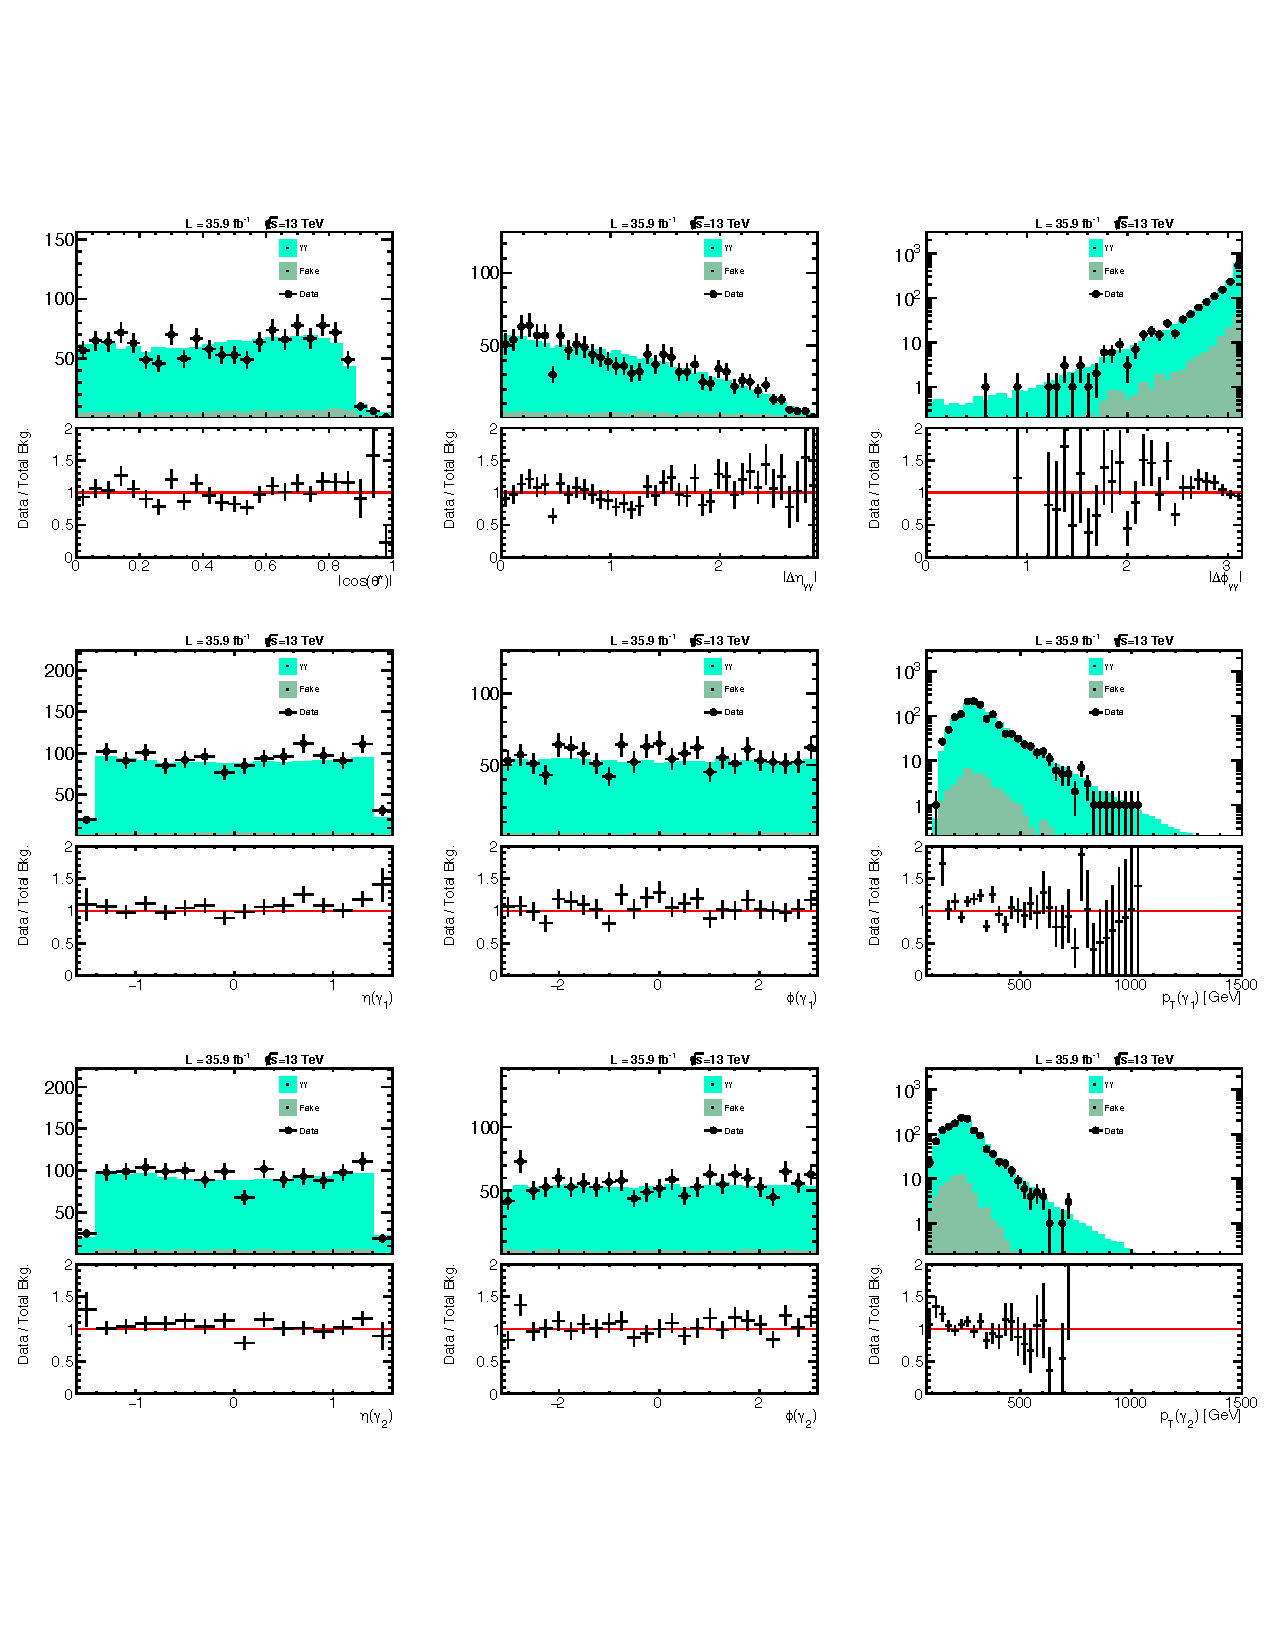
\includegraphics[width=1.0\textwidth]{figures/kinematicSummary_EBEB_merged.pdf}
	\caption{A comparison of various kinematic distributions between the SM background prediction, fake background measurement, and data. The photons are restricted to the EB and diphotons to the EBEB.}
	\label{fig:kinematics_EBEB}
\end{figure}

\begin{figure}[!htbp]
	\centering
	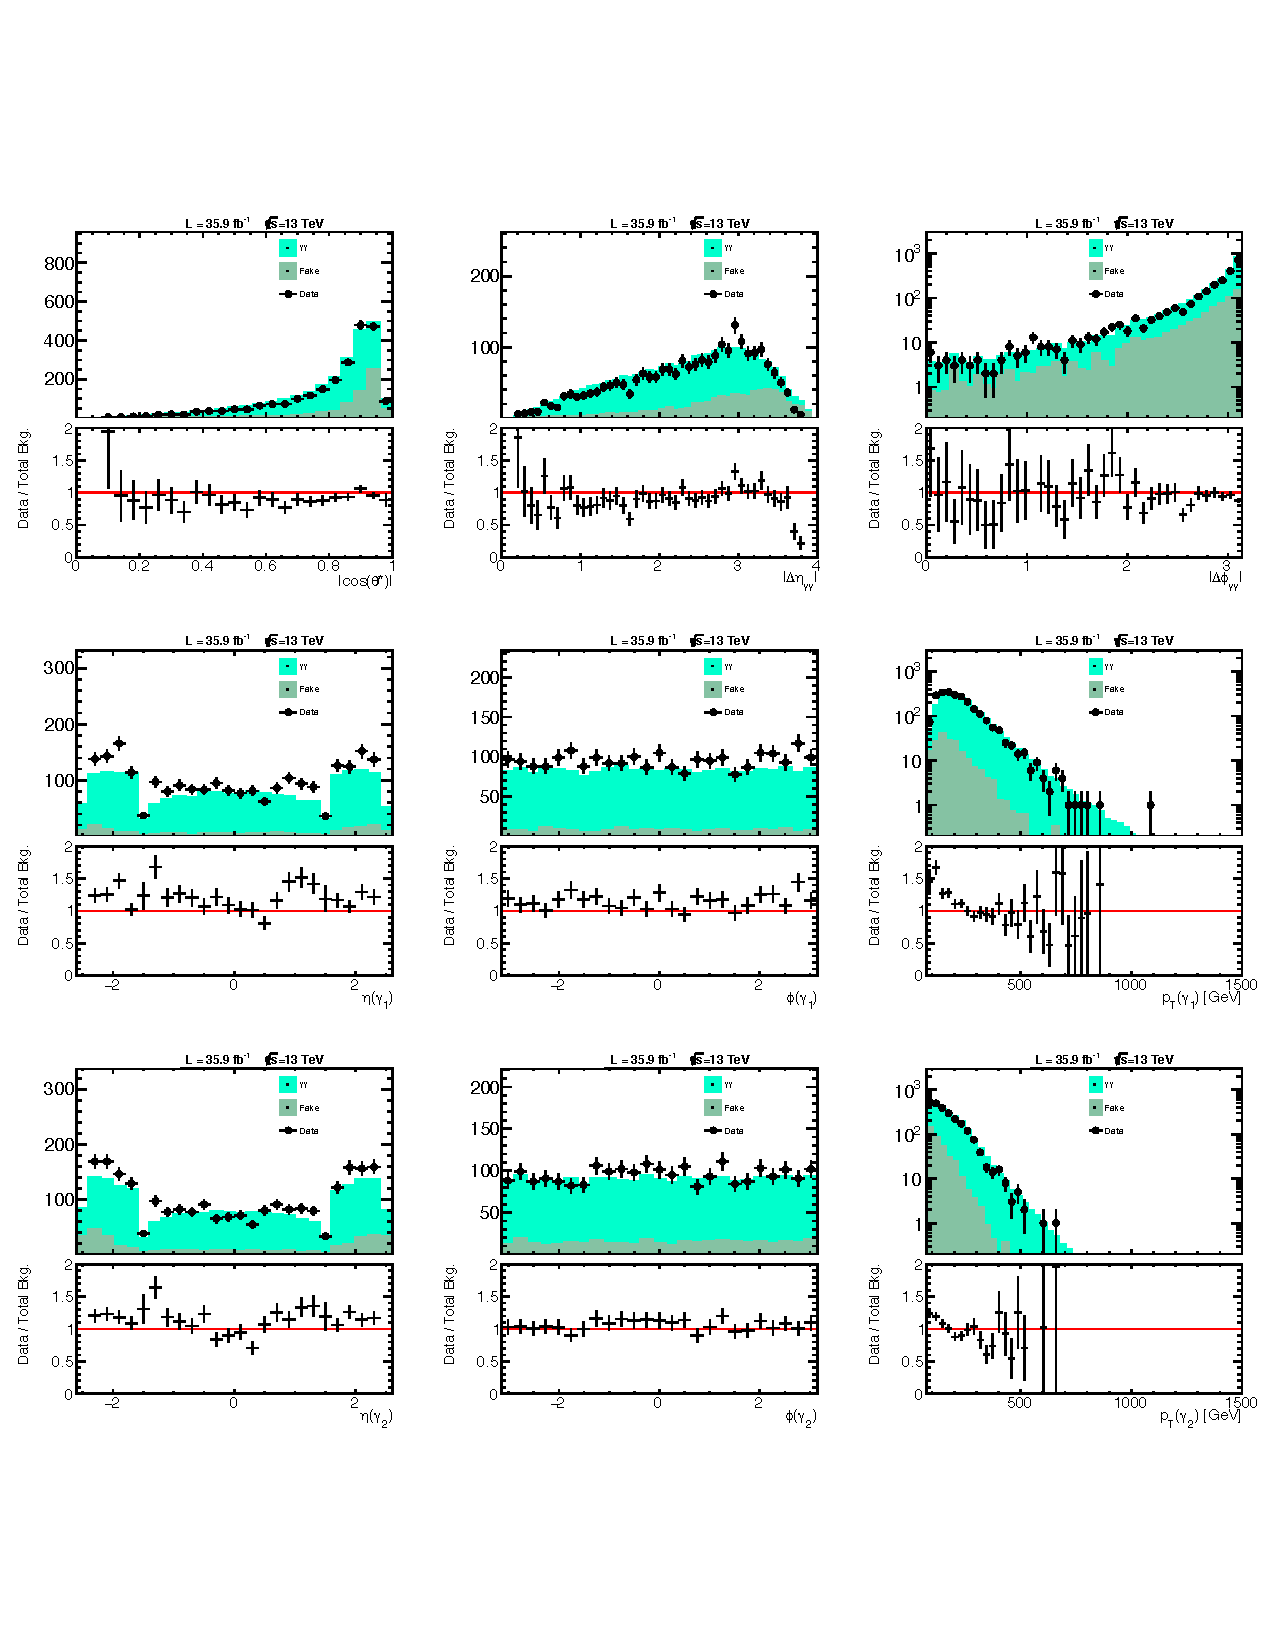
\includegraphics[width=1.0\textwidth]{figures/kinematicSummary_EBEE_merged.pdf}
	\caption{A comparison of various kinematic distributions between the SM background prediction, fake background measurement, and data. The photons are restricted to the EE and diphotons to the EBEE.}
	\label{fig:kinematics_EBEE}
\end{figure}


A list of the highest diphoton invariant mass \mgg events is provided in Table~\ref{tab:highest_mass_events}. No events containing photons causing saturation in the ECAL were observed. Fig.~\ref{fig:event_display} shows an event display of the highest invariant mass diphoton event recorded in 2016 at 1840\GeV in the EBEB category. The two photons in this event display are represented by the two large, red ECAL energy deposits. The highest diphoton invariant mass event in the EBEE category was recorded at 2444\GeV in 2016.

\begin{table}[!htbp]
	\scriptsize
	%\tiny
	\caption{The three highest \mgg events observed in data for the EBEB and EBEE categories. The photon \pt is given in units of {\GeVns}. The dataset paths begin with \texttt{/DoubleEG} and end with \texttt{/MINIAOD}, and include \texttt{X = 03Feb2017}. Here, run, LS, and event correspond to the run number, luminosity section, and event number, respectively. \correction{Each event was recorded in 2016, where pp collisions occurred (the majority of the time) from May-October.}}
	\label{tab:highest_mass_events}
	\centering
	\vspace{\baselineskip}
	\begin{tabular}{c|ccclll}
		\hline \hline
		%\vspace*{-4.5mm} & & & & & \\
		\vspace*{+0.1mm} & \mgg ({\GeVns}) & $\gamma_1$ (\pt, \scEta) & $\gamma_2$ (\pt, \scEta) & Run:LS:Event & Dataset path & Date \\
		\hline
		     & 1840.38 & (964.15, -0.881) & (429.01, 0.916) & 278820:832:1528641148 & /Run2016G-X-v1 & Aug 14 \\
		EBEB & 1816.31 & (833.60, -0.160) & (679.74, -1.424) & 276810:249:448659898 & /Run2016D-X-v1 & Jul 14 \\
		     & 1777.39 & (508.64, -1.053) & (451.83, 1.405) & 276437:452:753595848 & /Run2016D-X-v1 & Jul 6 \\
		\hline
     		 & 2444.38 & (415.88, -2.484) & (272.98, 1.442) & 279794:445:700510844 & /Run2016G-X-v1 & Aug 30 \\
		EBEE & 2134.42 & (570.82, -0.695) & (515.46, 1.916) & 284039:18:31148565 & /Run2016H-X\_ver3-v1 & Oct 26 \\
		     & 1985.68 & (577.69, -2.443) & (397.34, 0.273) & 276585:21:32975214 & /Run2016D-X-v1 & Jul 10 \\
		\hline \hline
	\end{tabular}
\end{table}

\begin{figure}[!htb]
  \centering
  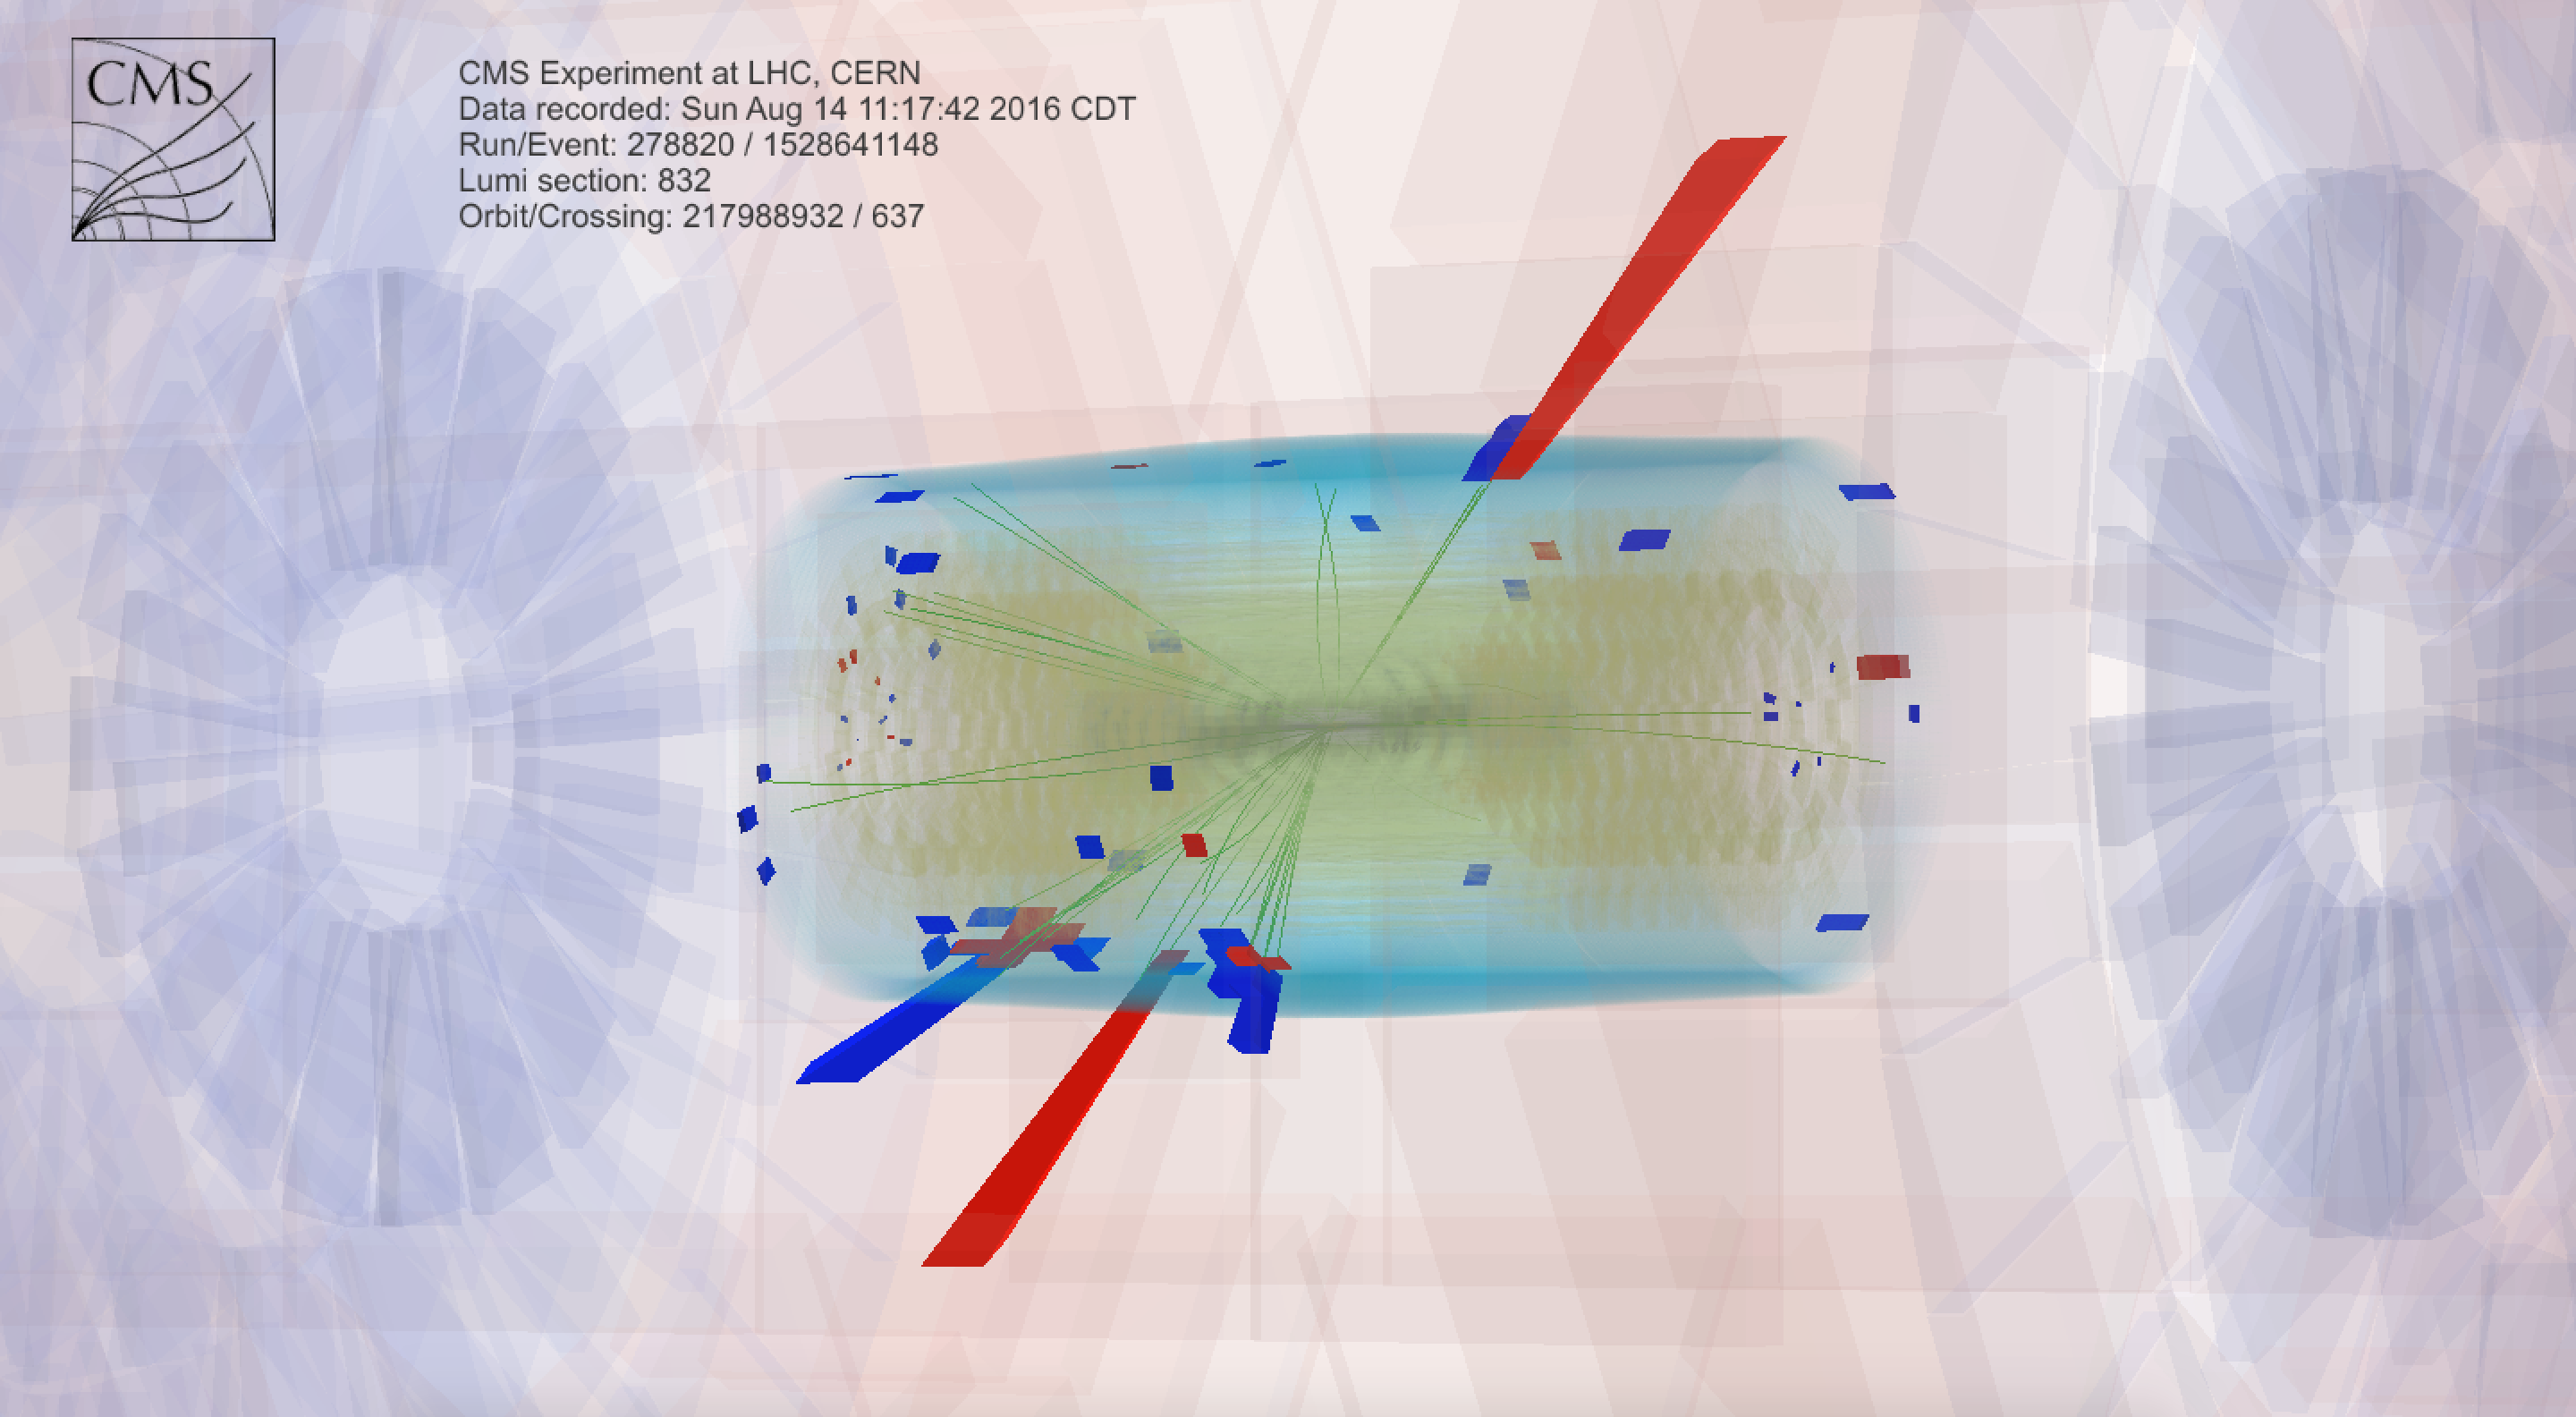
\includegraphics[width=0.99\textwidth]{figures/event_display_EBEB.png}
  \caption{An event display of the highest invariant mass diphoton event recorded in 2016 at 1840\GeV in the EBEB category. The two photons are represented by the two large, red ECAL energy deposits.}
  \label{fig:event_display}
\end{figure}

Further checks were performed on the high-mass diphoton events to ensure good health (e.g., to confirm that there was not large detector noise). The ($\eta,\phi$) spatial distribution of the events with $\mgg>1.5\TeV$ is shown in Fig.~\ref{fig:high_mass_eta_phi}, split between the leading and subleading photons in the EBEB and EBEE categories. \correction{The angular separation between the two photons is directly proportional to the \mgg of their associated diphoton object. Hence, these high-\mgg events tend to be back-to-back in the $\phi$ direction, as seen in the EBEB region.} The \rnine and \sieie distributions of these events are shown in Fig.~\ref{fig:high_mass_sieie_r9}, also split between the leading and subleading photons, but with both categories combined. Also, shown in this plot are the reference distributions obtained using all photons from events with $\mgg < 1.5\TeV$. These checks show that the high-mass diphoton events are compatible with the rest of the diphoton events, ensuring that they are genuine.

\begin{figure}[!hbt]
  \centering
  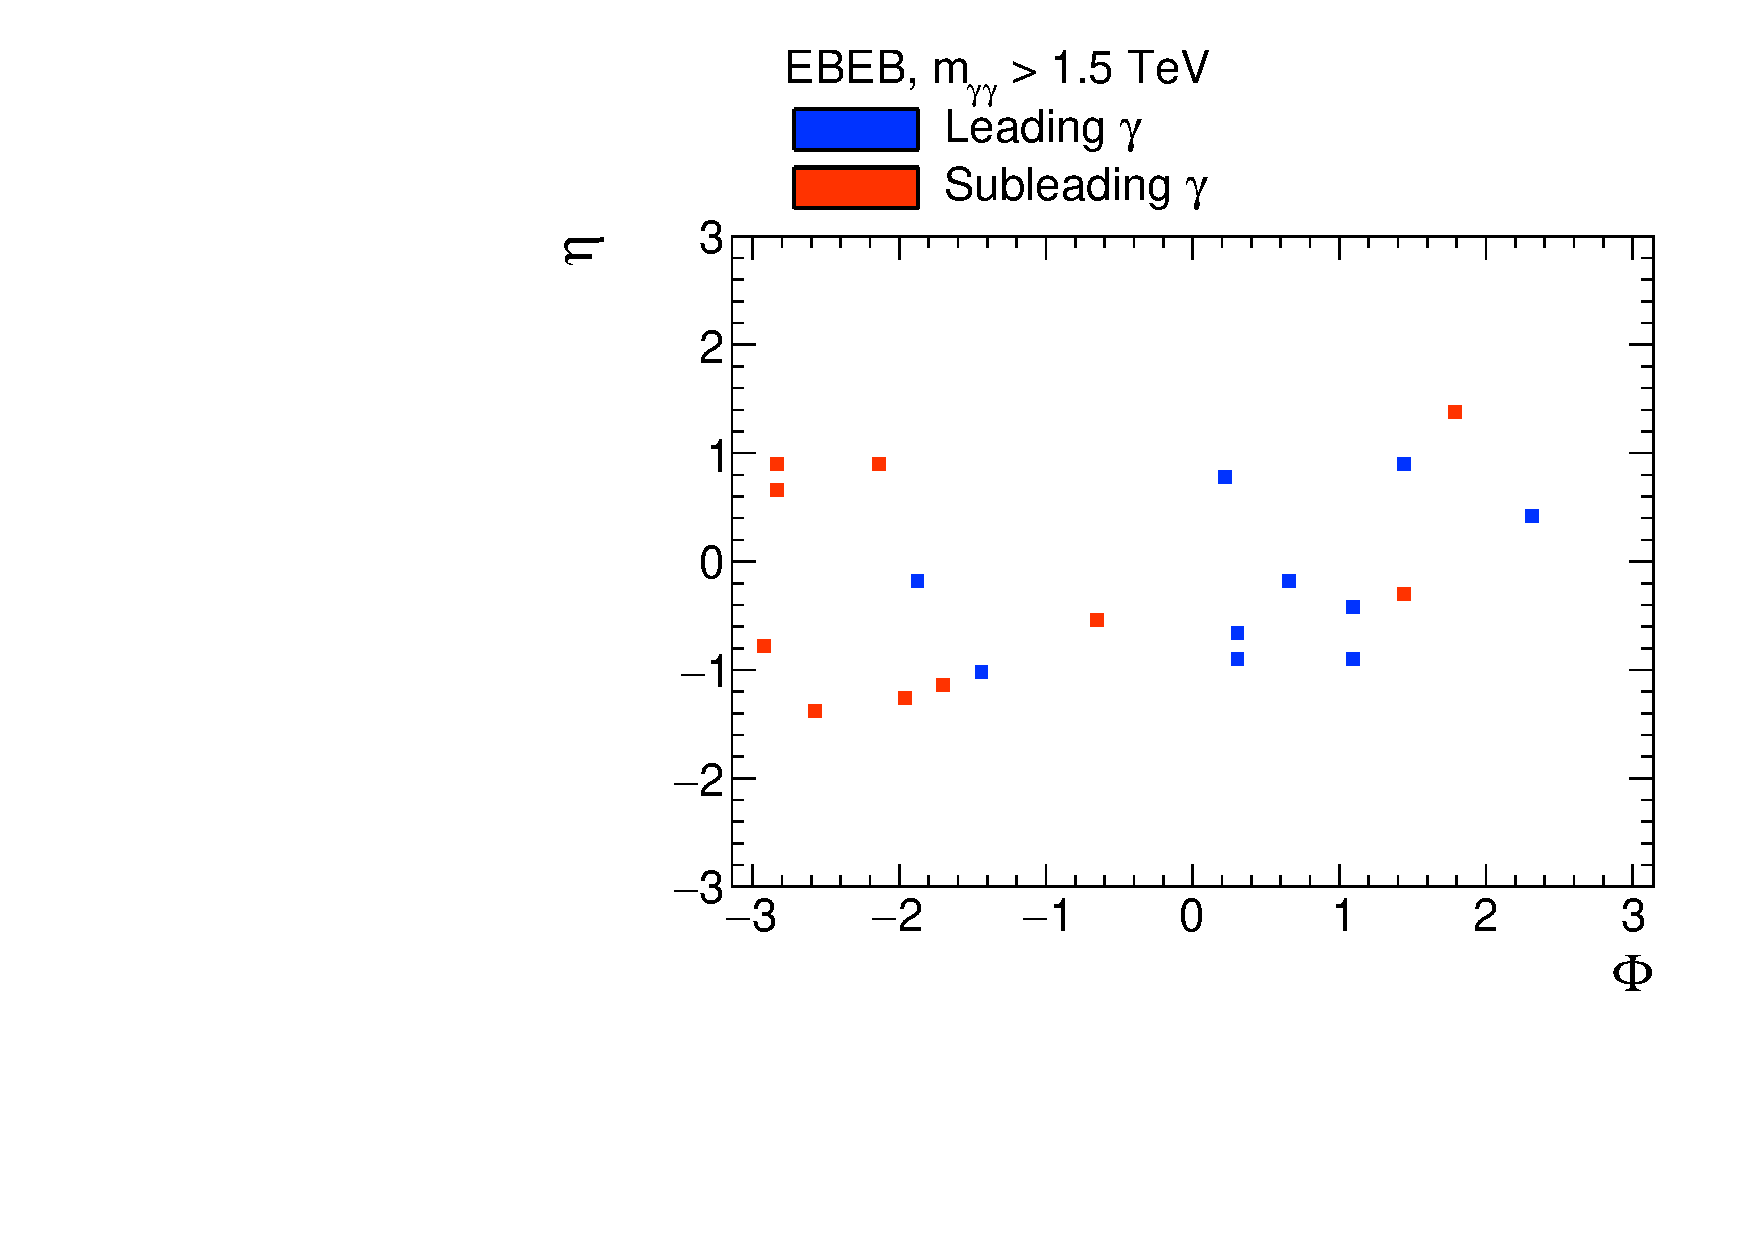
\includegraphics[width=0.45\textwidth]{figures/eta_phi_map_EBEB.pdf}
  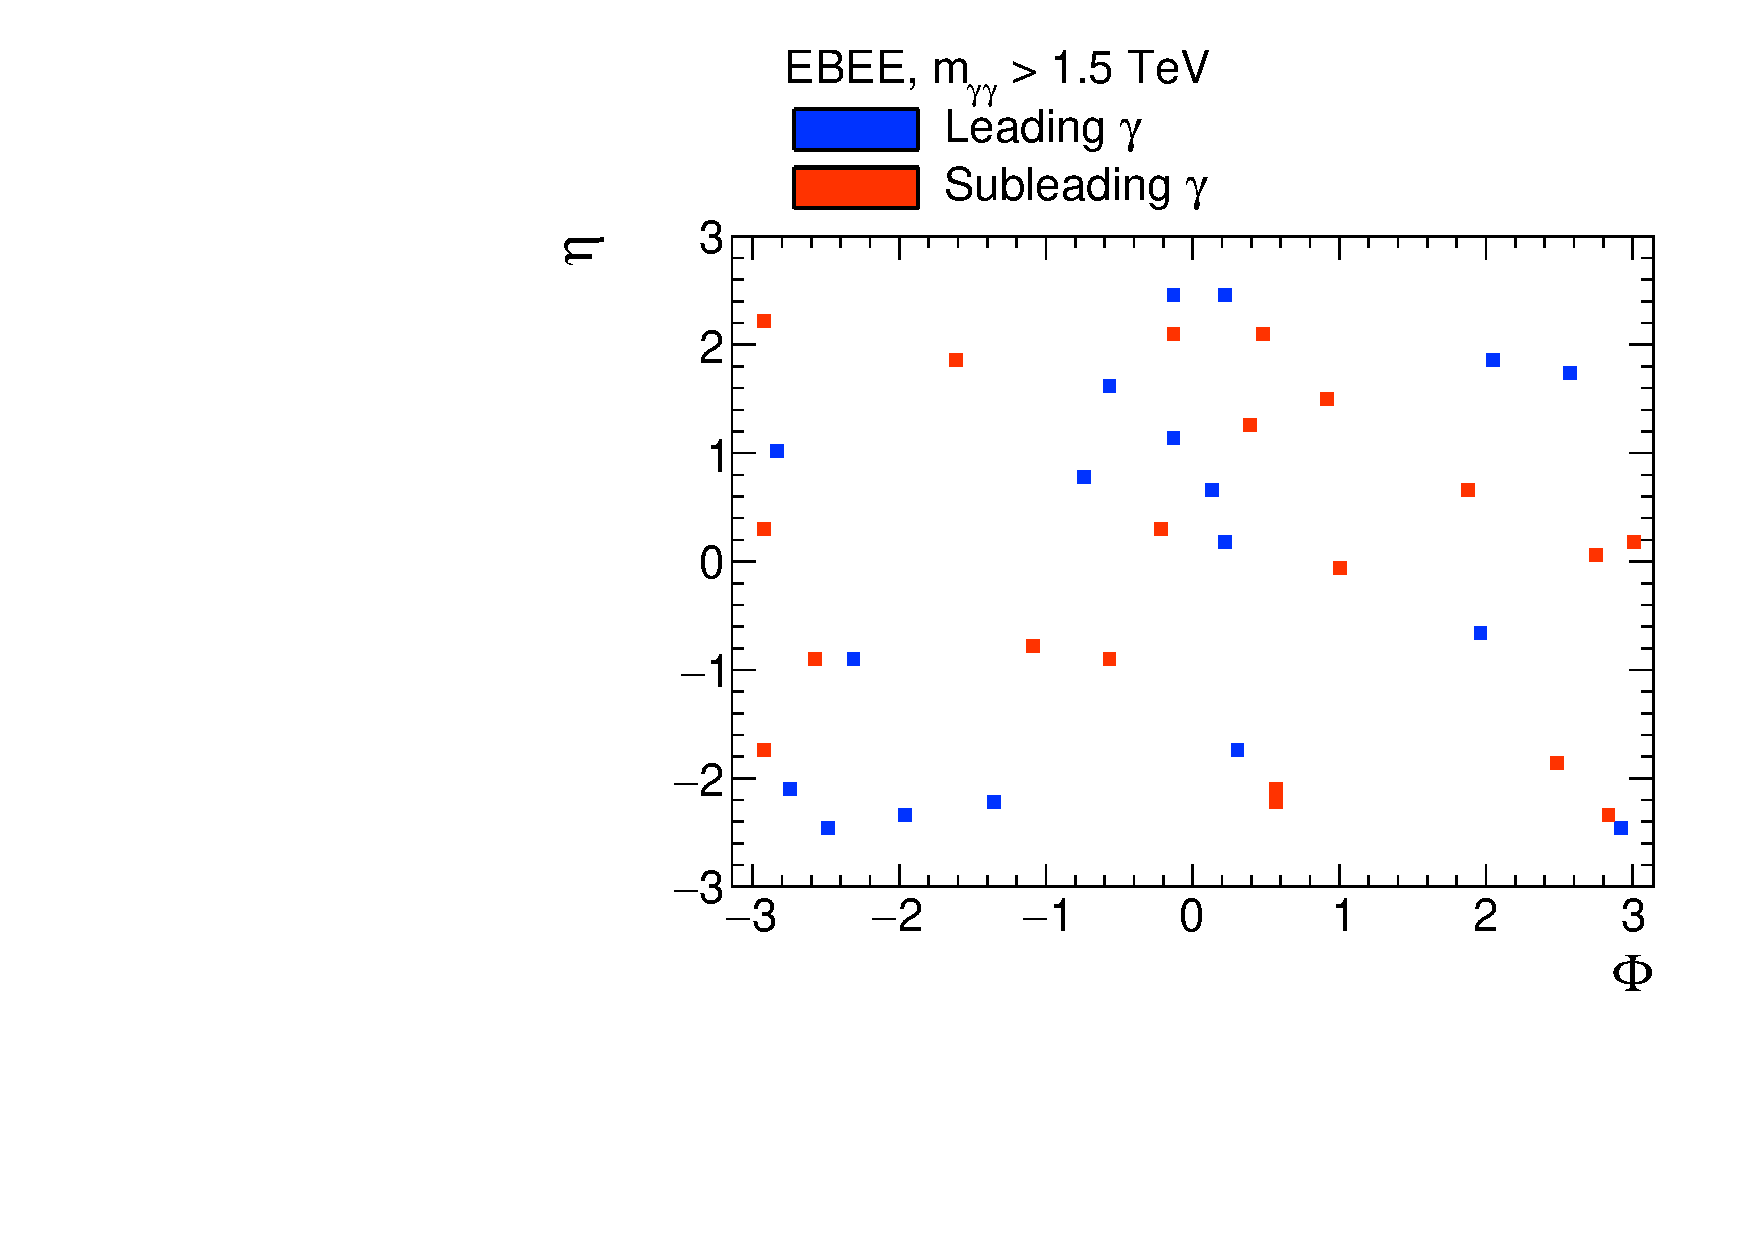
\includegraphics[width=0.45\textwidth]{figures/eta_phi_map_EBEE.pdf}
  \caption{The ($\eta,\phi$) spatial distribution of the leading (blue) and subleading (red) photons in the diphoton events with $\mgg>1.5\TeV$ for the EBEB (left) and EBEE (right) categories.}
  \label{fig:high_mass_eta_phi}
\end{figure}

\begin{figure}[!hbt]
  \centering
  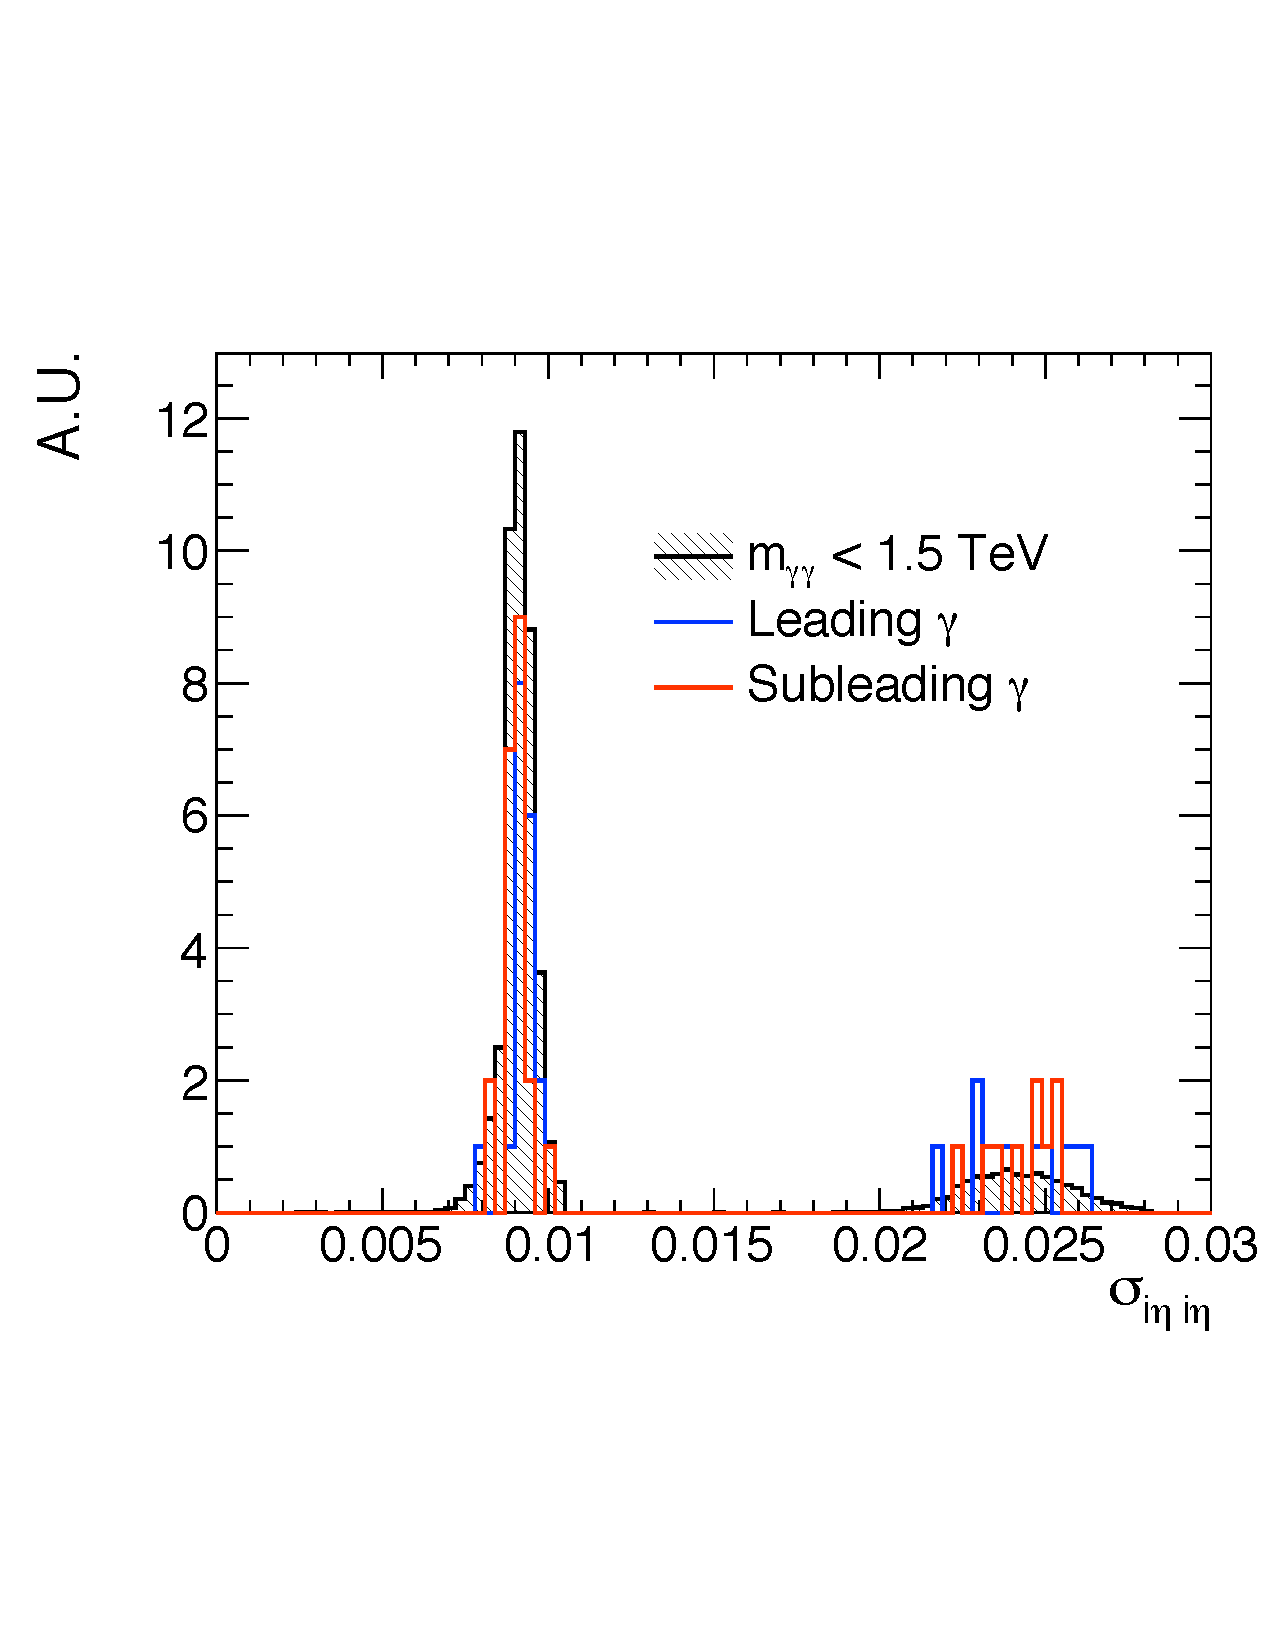
\includegraphics[width=0.45\textwidth]{figures/sieie_all_edit.pdf}
  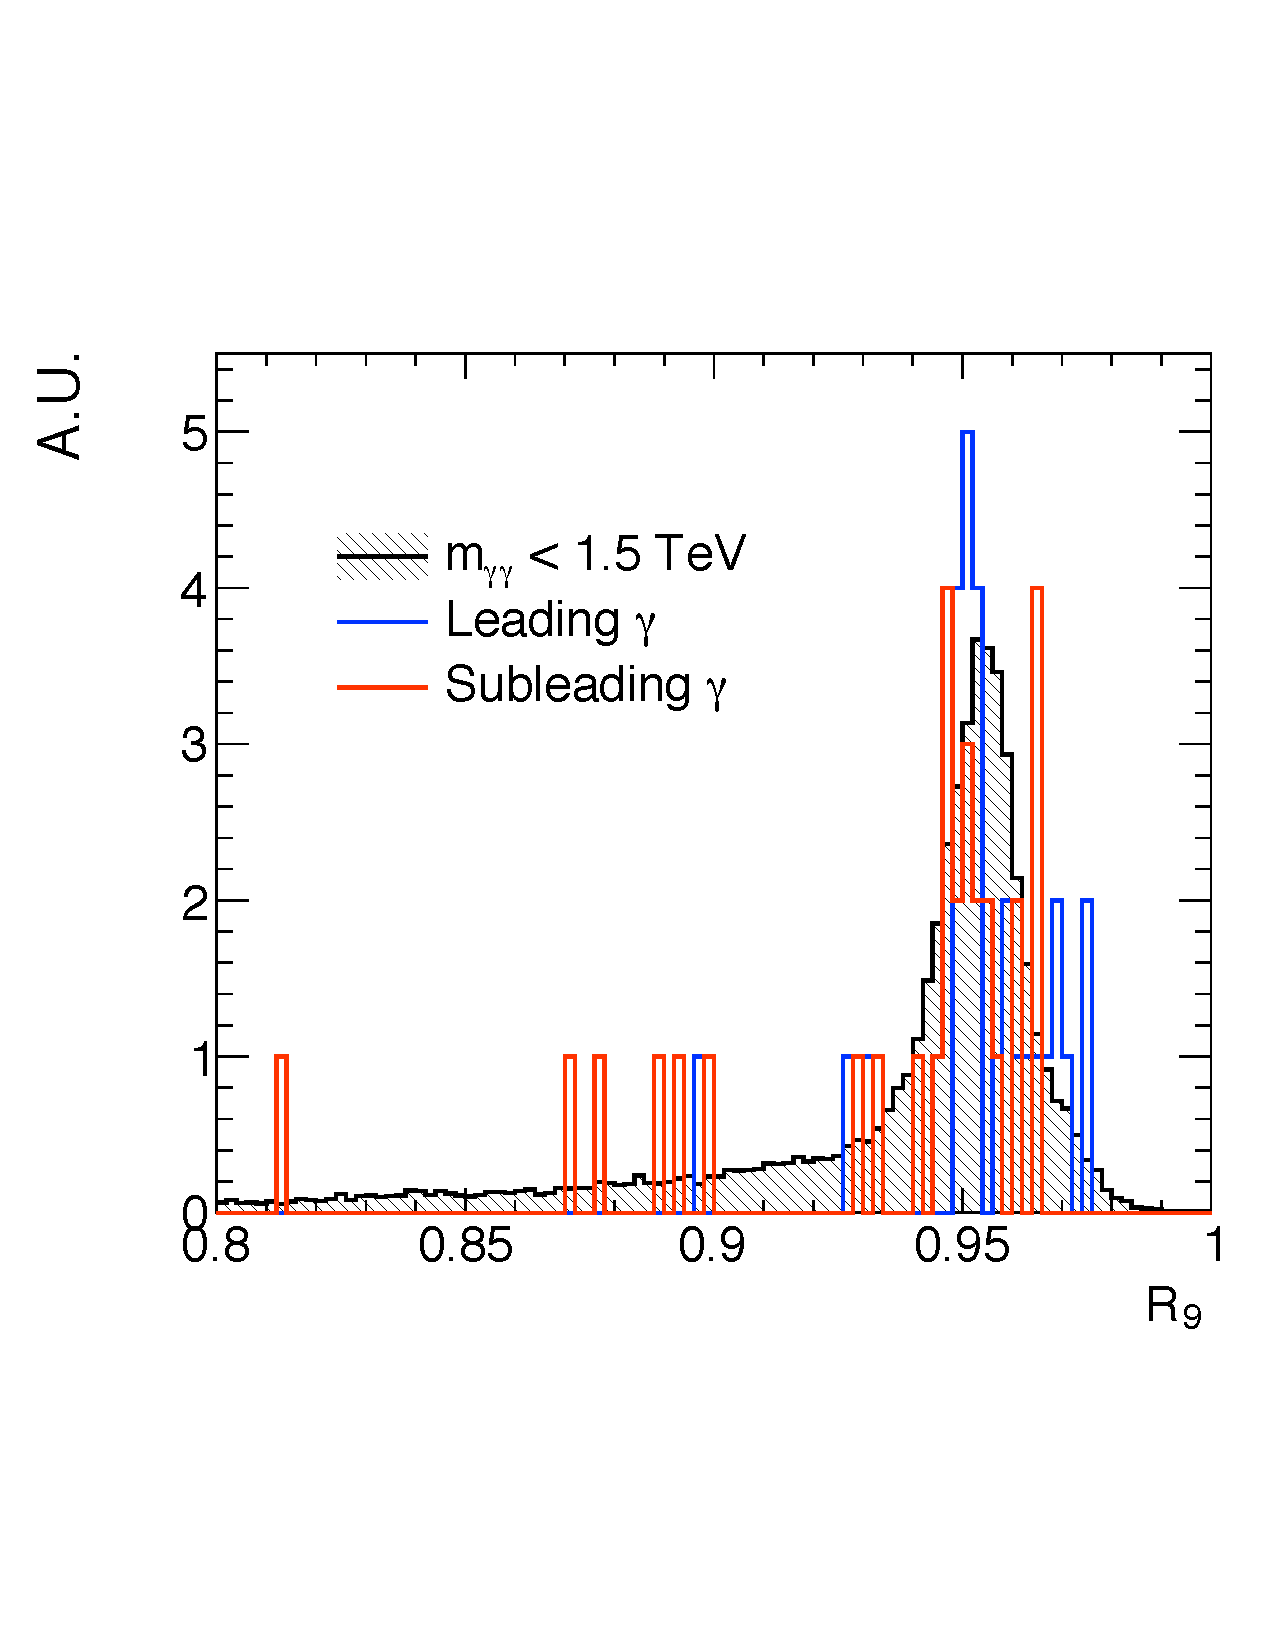
\includegraphics[width=0.45\textwidth]{figures/R9_all_edit.pdf}
  \caption{The \sieie (left) and \rnine (right) distributions of the leading (blue) and subleading (red) photons in the diphoton events with $\mgg>1.5\TeV$ compared to the photons in events with $\mgg < 1.5\TeV$. The $y$-axis is labeled using arbitrary units.}
  \label{fig:high_mass_sieie_r9}
\end{figure}

The final results are obtained in two stages: using the pre- and post-fit \mgg distributions from before and after the background normalization is allowed to float, respectively. These distributions utilize 100\GeV binning, starting at 500\GeV. Fig.~\ref{fig:mgg_pre_fit} shows the \mgg spectra using the pre-fit SM background prediction and the fake background measurement compared to the data in the EBEB and EBEE categories. The systematic uncertainties neglect the (unbounded) normalization of the diphoton prediction and the NLO shapes. Even though this does not constitute the final background prediction, excellent agreement is found, using the full NNLO background calculation. No significant excess of data over background is observed, as indicated in the bottom panels. These results are consistent with the background-only hypothesis for the signal search.

\begin{figure}[!htb]
  \centering
  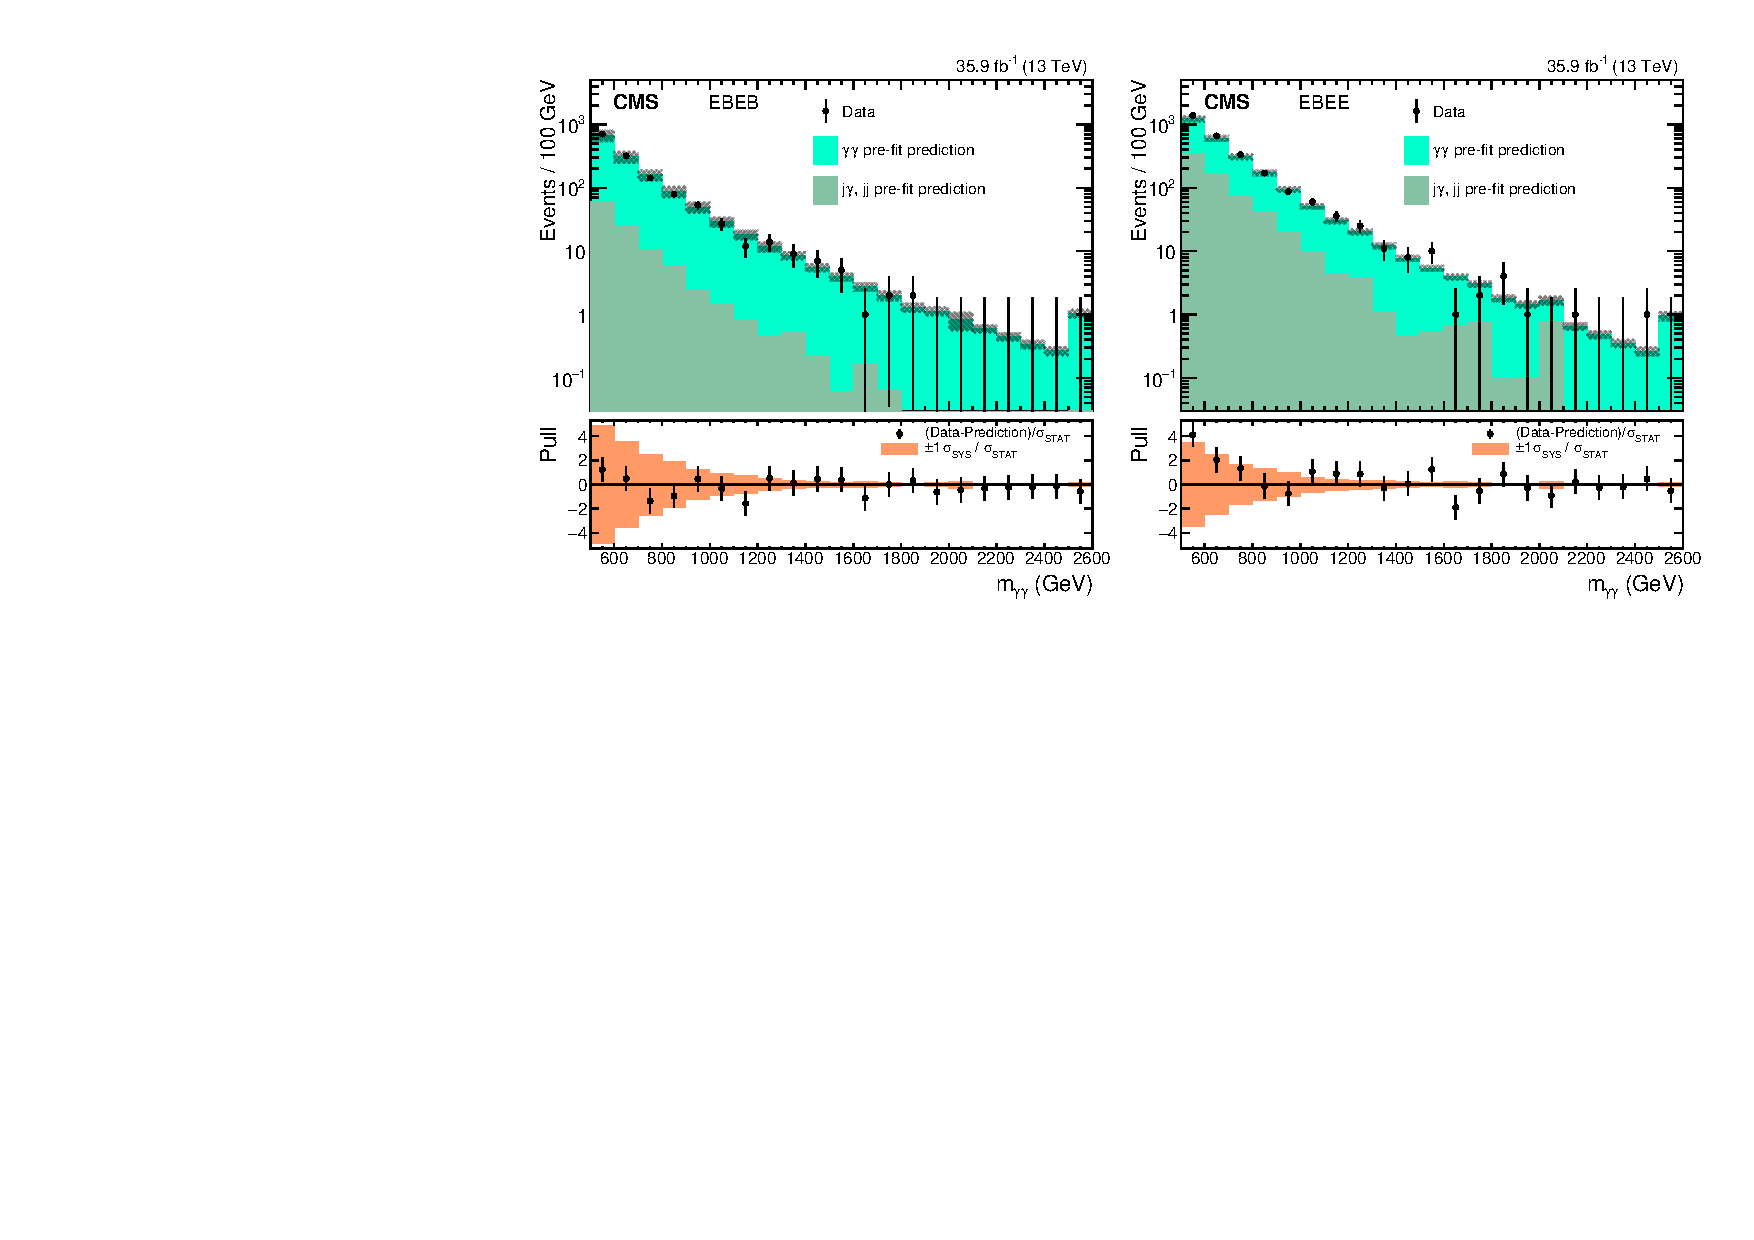
\includegraphics[width=1.0\textwidth]{figures/PLOT_PRED_PULL_35p9_0.pdf}
  \caption{The diphoton invariant mass distributions in the EBEB (left) and EBEE (right) categories for the pre-fit SM diphoton background prediction and the fake background measurement compared to the data. The last bin includes the overflow. The error bars on the points indicate the statistical uncertainty, and the hatched bands indicate the total pre-fit systematic uncertainties. The bottom panels show the pull distributions, indicating the difference between the data and background prediction, divided by the uncertainty in the background, with error bars representing the statistical uncertainty and shaded bands showing the one standard deviation systematic uncertainty, normalized by the statistical uncertainty.}
  \label{fig:mgg_pre_fit}
\end{figure}

The final post-fit prediction is performed simultaneously with the limit extraction on the ADD model parameters. A Bayesian statistical approach is adopted and performed by the \textsc{theta} framework~\cite{theta}. The systematic uncertainties described in Chapter~\ref{ch:systematics} are treated as nuisance parameters and are marginalized using a Markov chain MC method~\cite{Metropolis:1953am} within \textsc{theta}. After the marginalization of the nuisance parameters, posterior predictions for the SM background \mgg spectra are derived, using the data as a constraint. Since this fit is performed simultaneously with the limit setting procedure, the process will be detailed in the next section, during the limit setting discussion.

Fig.~\ref{fig:mgg_post_fit} shows the final post-fit predictions of the SM background and the fake background measurement compared to the data in the EBEB and EBEE categories. As is the case with the pre-fit prediction, excellent agreement is found within the total uncertainty. As expected, the uncertainties on the post-fit prediction are smaller. The invariant mass distributions from the ADD signal scenario using the HLZ convention assuming $\nED=2$ and $\Ms=8\TeV$ are superimposed. The highest diphoton invariant mass events probed are 1840 and 2444\GeV in the EBEB and EBEE categories, respectively. A breakdown of the event yields for the total pre- and post-fit background predictions compared to the data are listed in Table~\ref{tab:event_yields}, using different ranges of \mgg.

\begin{figure}[!htbp]
  \centering
  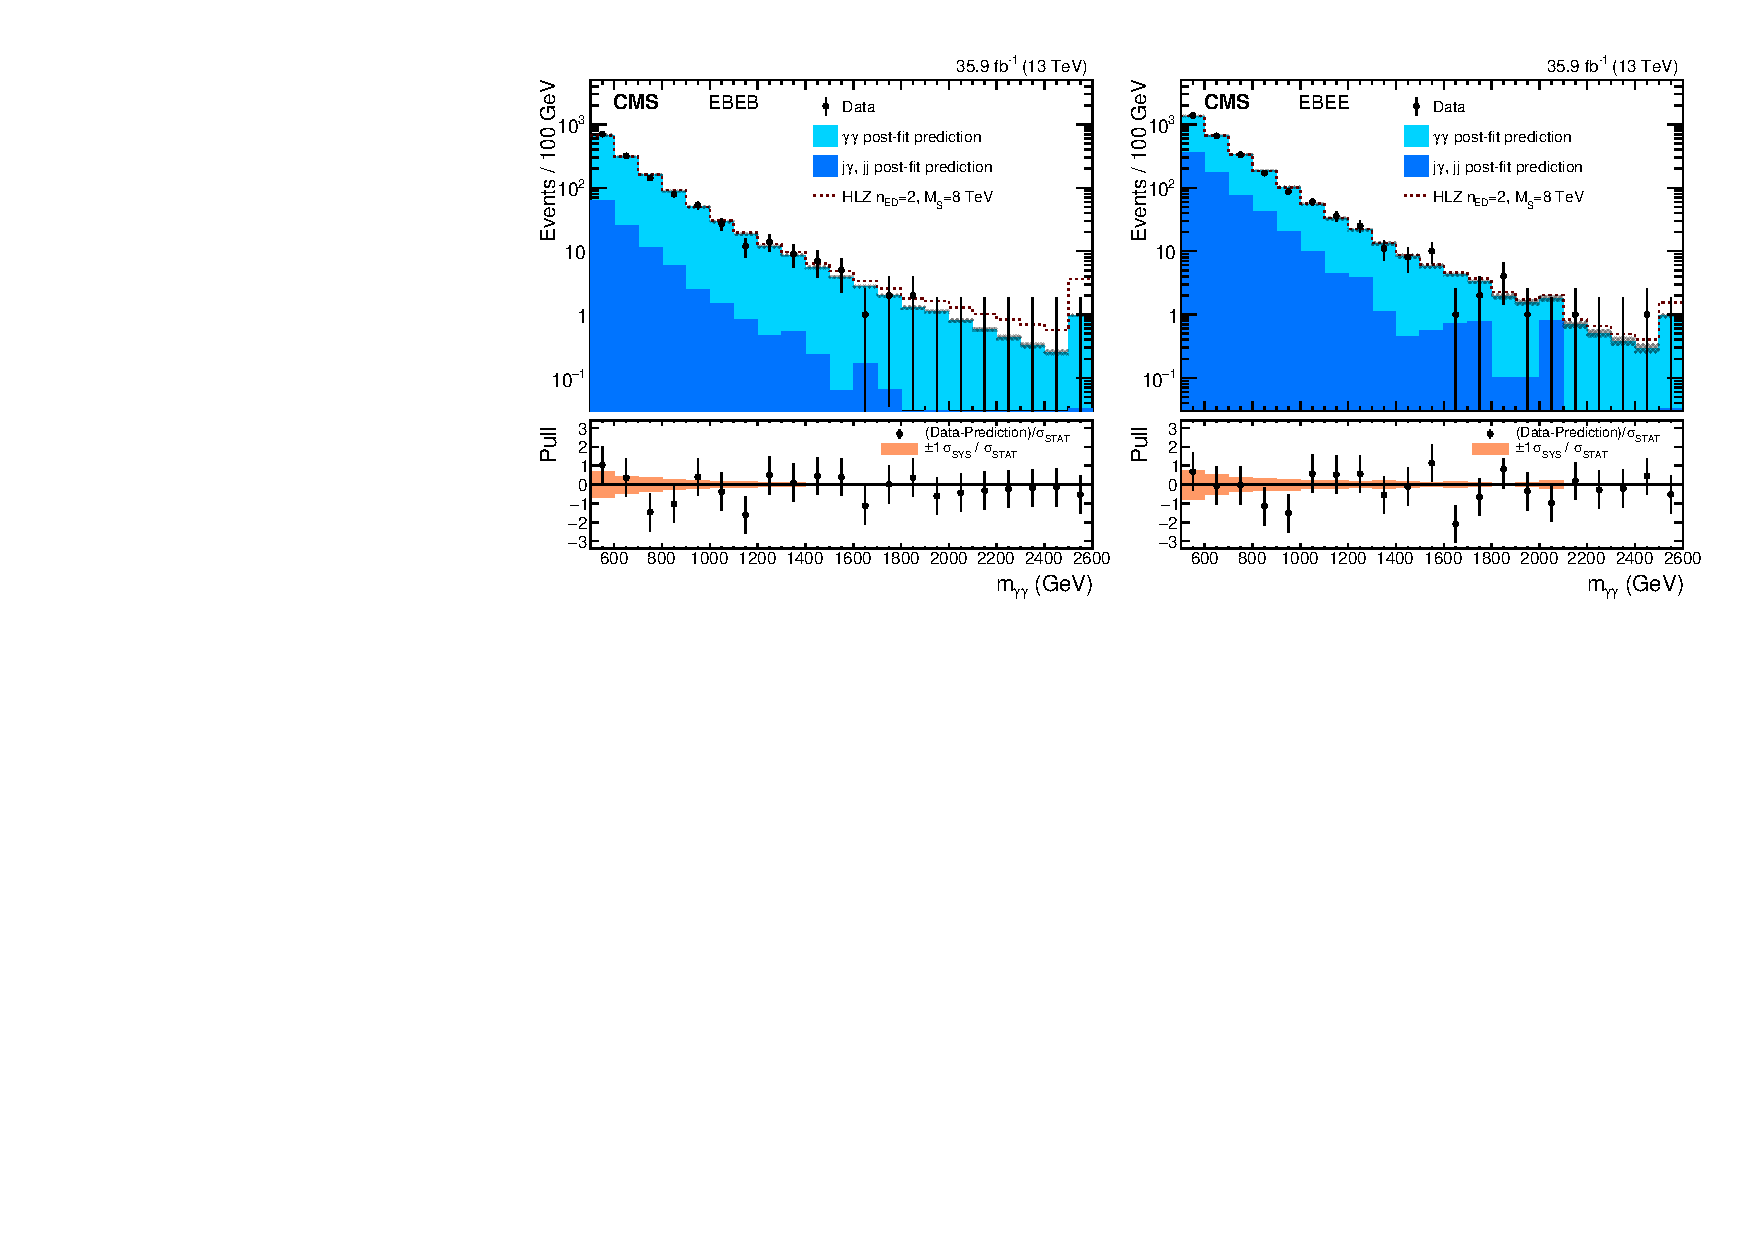
\includegraphics[width=1.0\textwidth]{figures/PLOT_PRED_PULL_35p9_1_no_clockwork.pdf}
  \caption{The diphoton invariant mass distributions in the EBEB (left) and EBEE (right) categories for the post-fit SM diphoton background prediction and the fake background measurement compared to the data. The last bin includes the overflow. The error bars on the points indicate the statistical uncertainty, and the hatched bands indicate the total post-fit systematic uncertainties. Invariant mass distributions from one signal scenario is superimposed. The bottom panels show the pull distributions, indicating the difference between the data and background prediction, divided by the uncertainty in the background, with error bars representing the statistical uncertainty and shaded bands showing the one standard deviation systematic uncertainty, normalized by the statistical uncertainty.}
  \label{fig:mgg_post_fit}
\end{figure}

\begin{table}[!htbp]
	\footnotesize %\scriptsize
	\caption{Event yields for the total pre- and post-fit background predictions compared to the data for different ranges of \mgg. The total systematic uncertainties are included on the post-fit yields.}
	\label{tab:event_yields}
	\centering
	\vspace{\baselineskip}
	\begin{tabular}{cc|cccc|c}
		\hline \hline
		Category & Type & 0.5-1\TeV & 1-1.5\TeV & 1.5-2\TeV & 2-13\TeV & 0.5-13\TeV \\ 
		\hline
		&  Total pre-fit background & 1275.7 & 73.0 & 11.1 & 3.5 & 1363.3 \\ 
		EBEB & Total post-fit background & $1285\pm40$ & $73.7\pm2.9$ & $11.0\pm0.5$ & $3.30\pm0.22$ & $1373.0\pm40.1$ \\ 
		& Data & 1296 & 69 & 10 & 0 & 1375 \\ 
		\hline
		& Total pre-fit background & 2406.1 & 121.4 & 15.6 & 4.4 & 2547.5 \\ 
		EBEE & Total post-fit background & $2645\pm60$ & $128\pm6$ & $16.1\pm1.2$ & $4.1\pm0.5$ & $2793.2\pm60.3$ \\ 
		& Data & 2631 & 140 & 18 & 2 & 2791 \\ 
		\hline \hline
	\end{tabular}
\end{table}

\pagebreak


\section{Limits on the ADD Model}\label{sec:limit_setting}

Bayesian inference is used for setting upper limits on the ADD signal model parameters based on the background measured and data. An overview of general statistical methods can be found in Section~39 of Ref.~\cite{Tanabashi:2018oca} and in Ref.~\cite{Cousins:2018tiz}, and a general prescription of statistical applications to CMS searches can be found in Ref.~\cite{CMS-NOTE-2011-005}. The Bayesian approach used here follows the procedure described in Ref.~\cite{Bertram:2000br}.

Given some prior degree of belief in a hypothesis for an experimental measurement, the probability for a given event to occur can be inferred through Bayes' theorem:
\begin{equation}
	P(A|B) = \frac{P(B|A) P(A)}{P(B)}
\end{equation}
for some hypothesis $A$ given event $B$ with $P(B)\ne 0$. $P(A)$ is the prior probability of $A$, $P(A|B)$ is the posterior probability of $A$ given $B$, $P(B|A)$ is the likelihood of $B$ given $A$, and $P(B)$ is sometimes called the marginal likelihood of $B$. \correction{For this limit-setting procedure, a binned likelihood is constructed such that the total likelihood $\mathcal{L}$ is equal to the product of the individual likelihoods $\mathcal{L}_i$ in each bin $i$. Given the counting nature of the experiment, the likelihoods take on the following Poissonian form:}
\begin{equation}
	\mathcal{L}(n|s,b) = \prod_{i} \mathcal{L}_i(n_i|s_i,b_i) =  \prod_{i} \frac{(s_i + b_i)^{n_i}e^{-(s_i + b_i)}}{n_i!}
\end{equation}
\correction{where $n$, $s$, and $b$ are the total number of data, signal, and background events, respectively, and the subscript on these quantities denotes the number of them in bin $i$. Substituting this into Bayes' theorem, we recast its form as}
\begin{equation}
	P(s,b|n) = \frac{\mathcal{L}(n|s,b)\pi(s,b)}{P(n)} = \mathcal{L}(n|s,b)\pi(s,b)
\end{equation}
\correction{where $P(n)$ is treated as a normalization constant and has been absorbed into the likelihood. By convention in the field, a flat prior $\pi(s,b)$, bounded below by zero, is assumed for each ADD signal model considered.}

\correction{The signal and background depend on their associated systematic uncertainties, which are each assigned a separate nuisance parameter $\theta$. For each nuisance parameter, a choice of prior $\pi(s,b,\theta)$ is made. These are handled by integrating them out in the following way:}
\begin{equation}
	P(s,b|n) = \int P(s,b,\theta|n) d\theta = \int \mathcal{L}(n|s,b,\theta)\pi(s,b,\theta)d\theta
\end{equation}
\correction{The prior shapes for each systematic uncertainty are either lognormal or Gaussian, depending on whether or not the uncertainty is bounded below by zero, except for the diphoton background normalization, which has a flat prior, motivated by our lack of prior knowledge on its uncertainty and due to this being a shape analysis. The posterior distributions for all nuisance parameters together with their $\pm1$ standard deviation variations in the EBEB and EBEE categories are shown in Figs.~\ref{fig:Multi_PDFs_A}, \ref{fig:Multi_PDFs_B}, and~\ref{fig:Multi_Rest}. As seen in these figures, when the prior is Gaussian, its posterior distribution is largely unmodified and remains Gaussian, especially for the nuisance parameters associated with the PDF eigenvectors.}

\begin{figure}[!htbp]
	\centering
	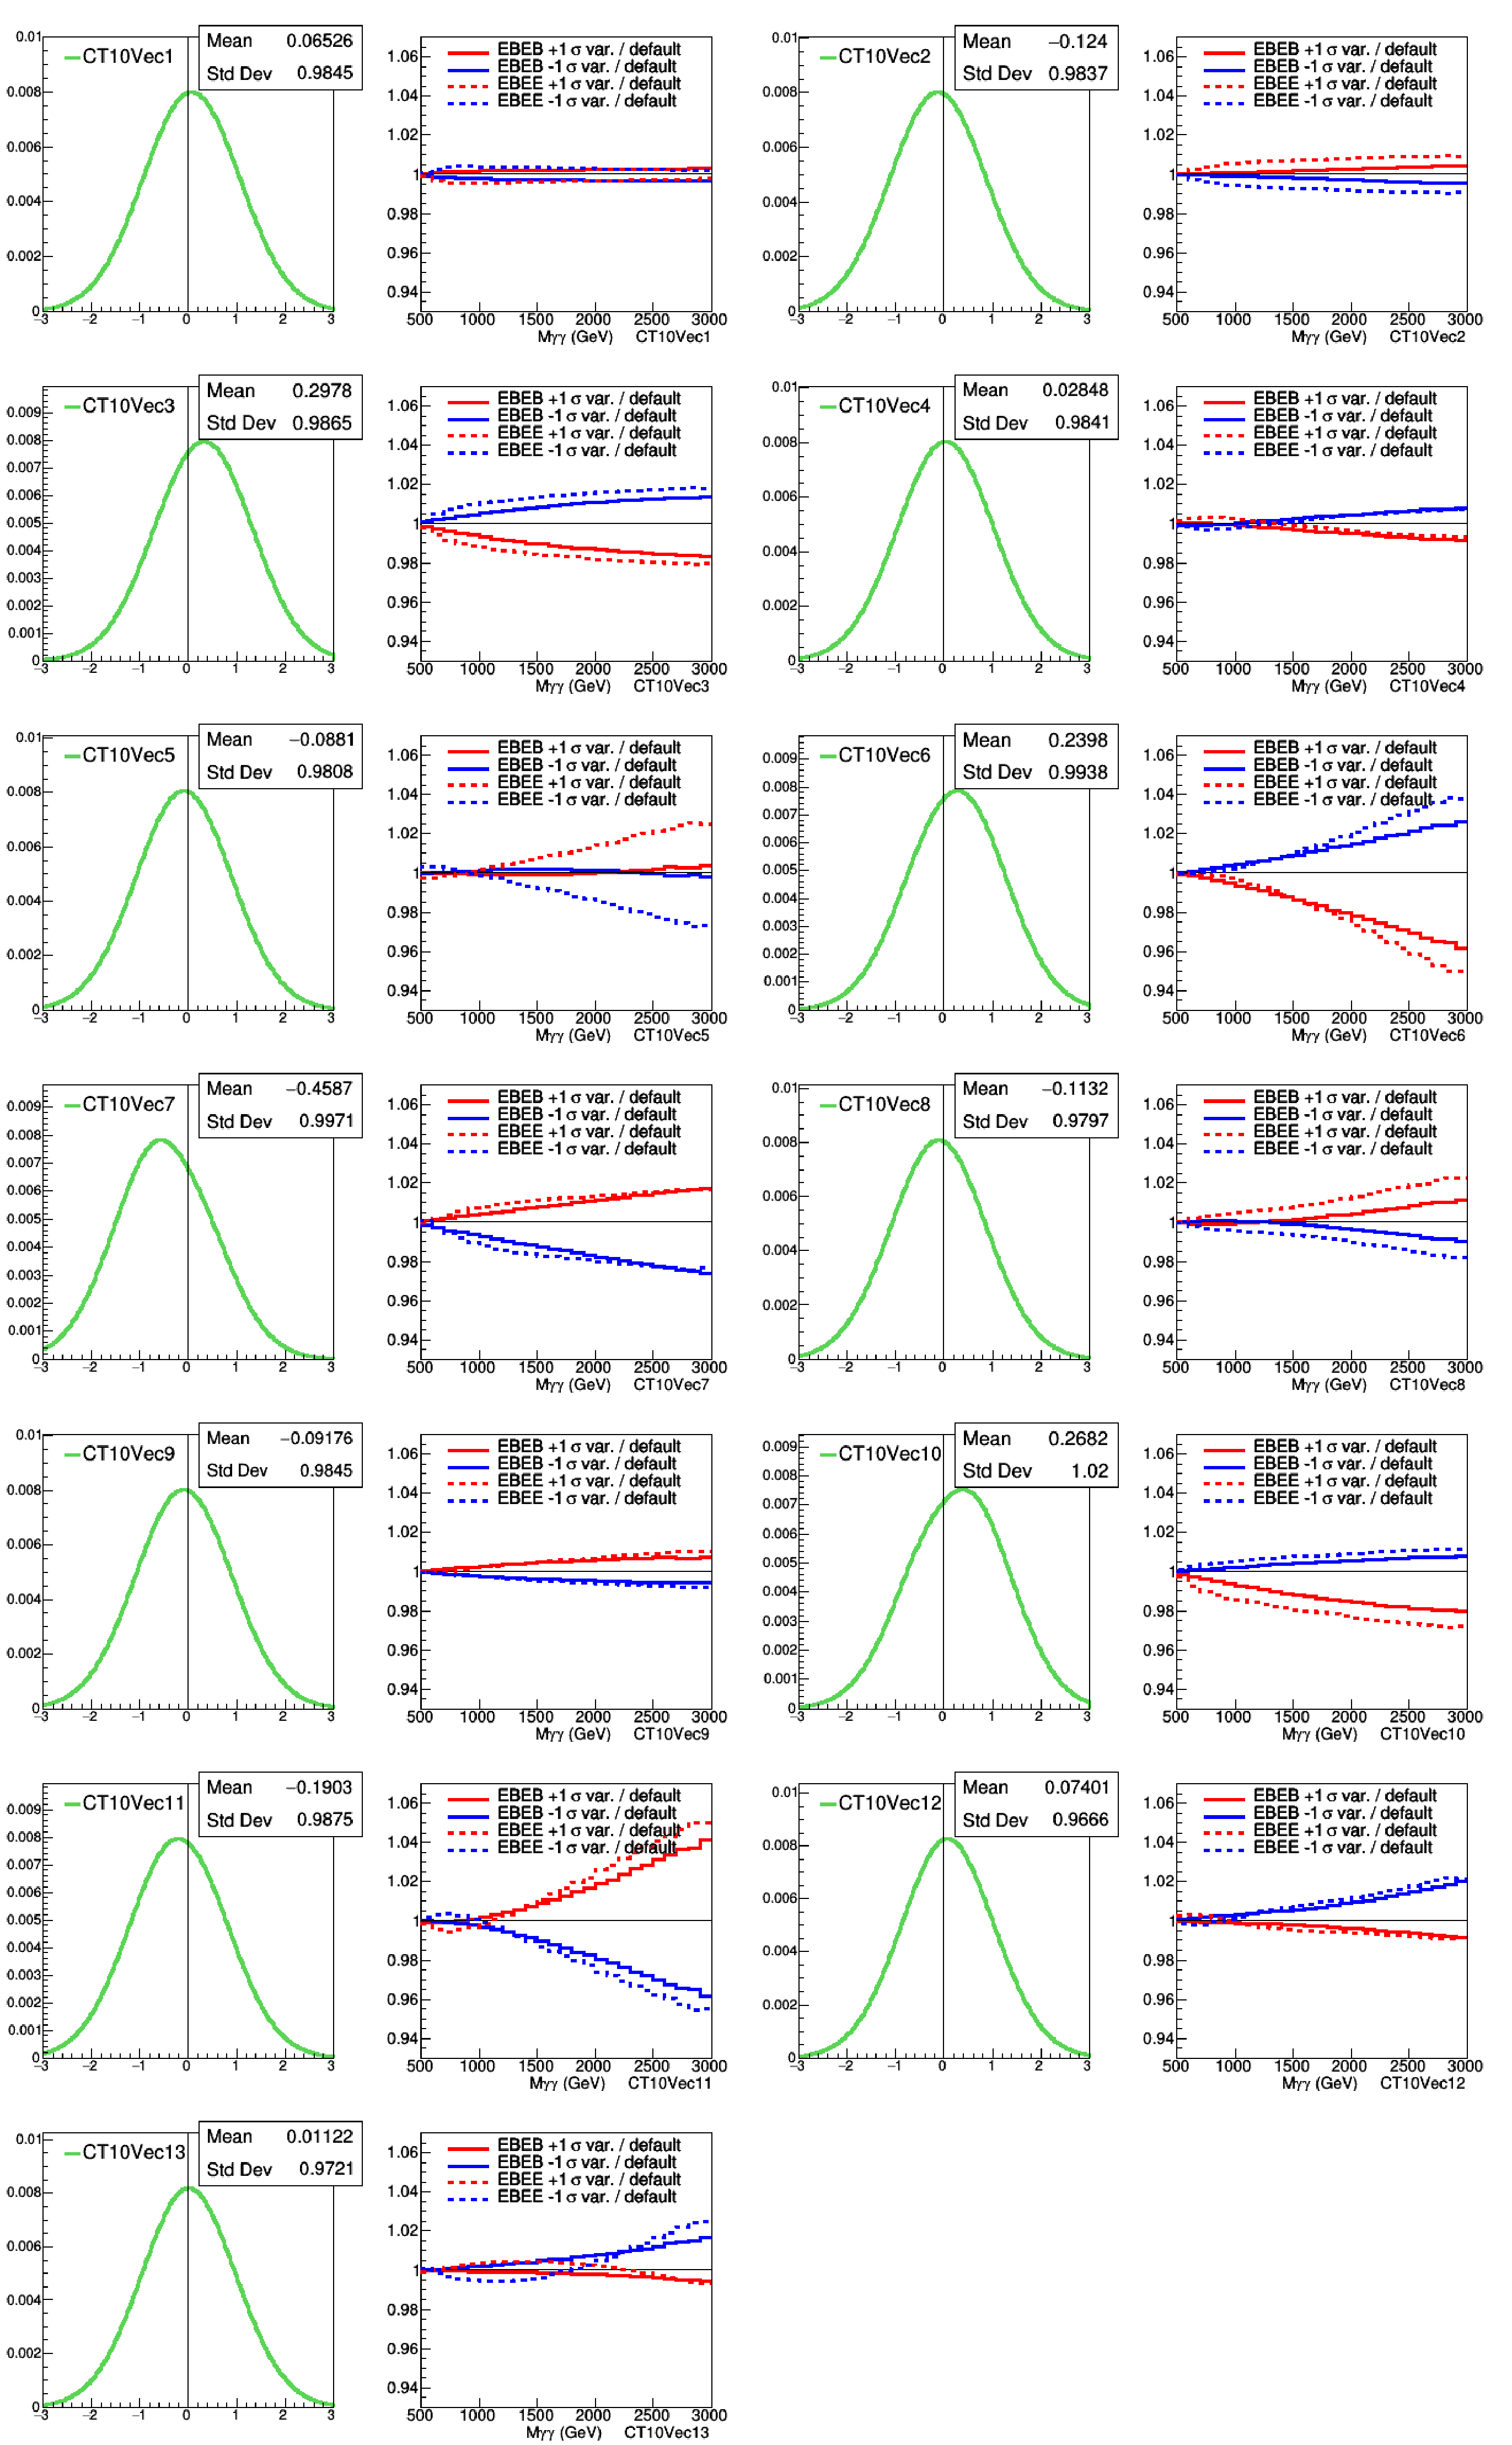
\includegraphics[scale=0.26]{figures/Multi_PDFs_A.pdf}
	\caption{Posterior Gaussian distributions (using a mean of 0 and standard deviation of 1) of the nuisance parameters assigned to PDF eigenvectors 1-13 (first and third columns). Their $\pm1$ standard deviation variations are shown as a ratio of the variation over the default prediction as a function of \mgg in the EBEB (solid) and EBEE (dashed) categories (second and fourth columns).}
	\label{fig:Multi_PDFs_A}
\end{figure}

\begin{figure}[!htbp]
	\centering
	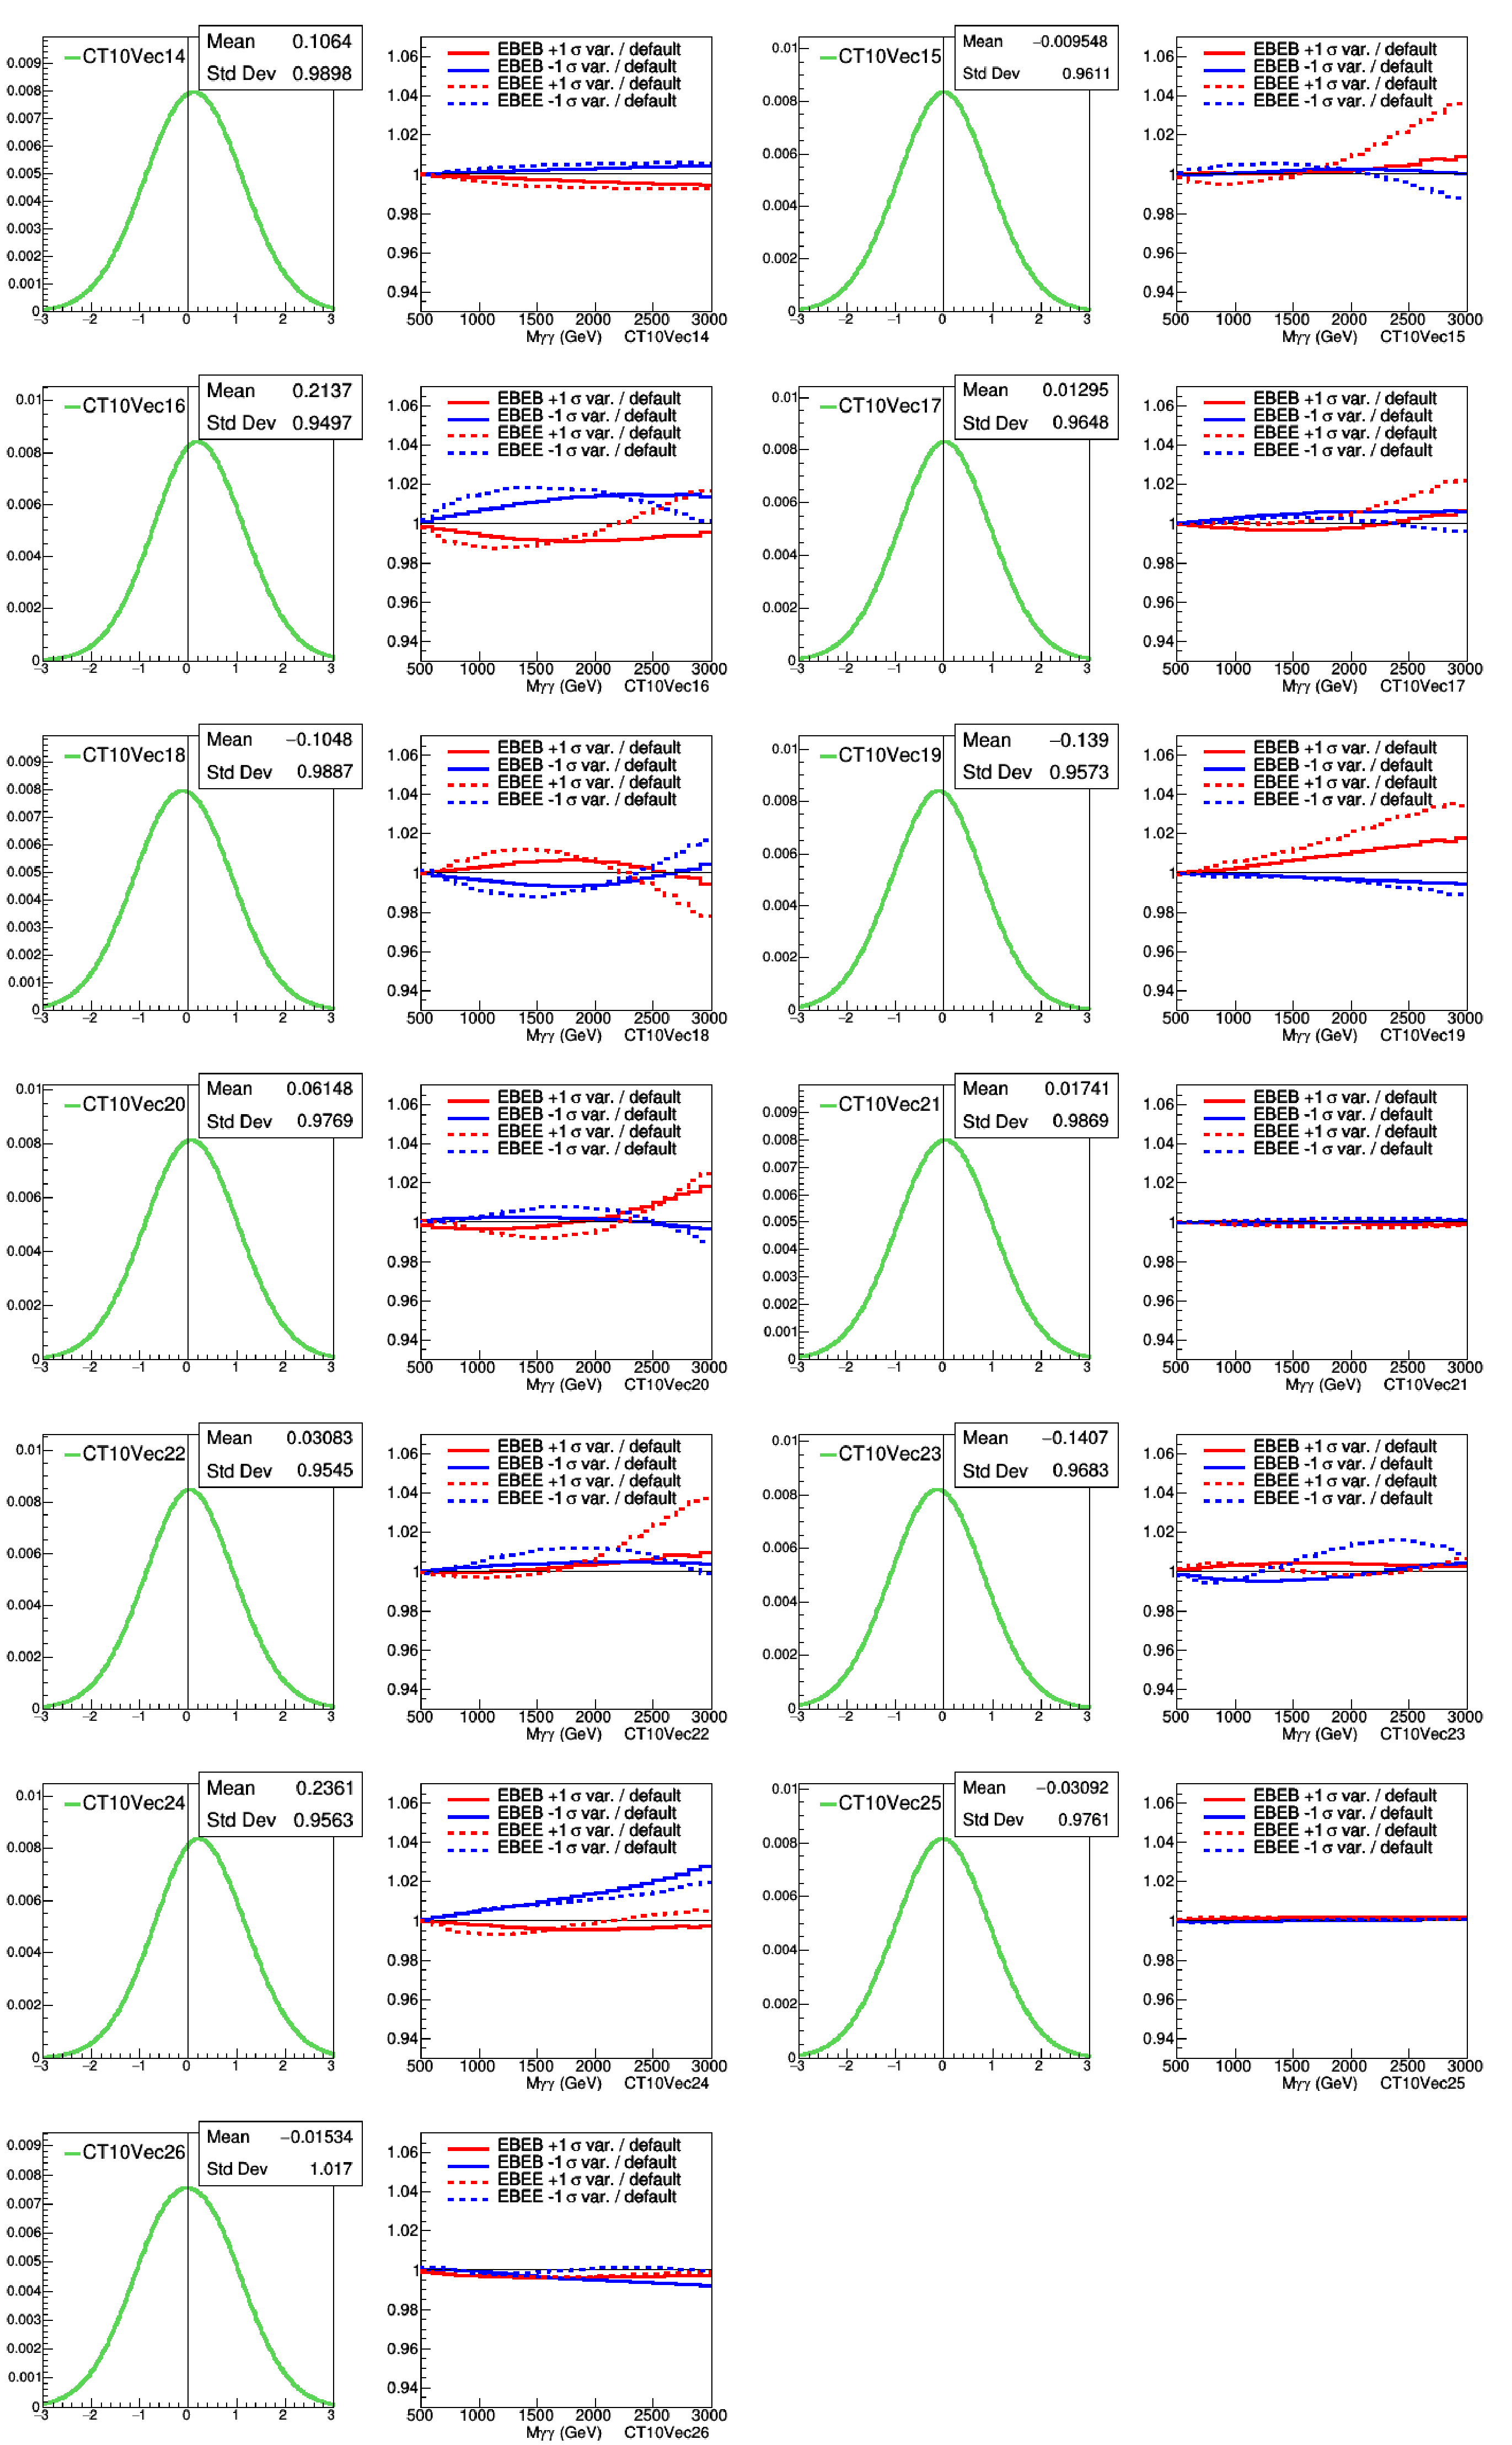
\includegraphics[scale=0.26]{figures/Multi_PDFs_B.pdf}
	\caption{Posterior Gaussian distributions (using a mean of 0 and standard deviation of 1) of the nuisance parameters assigned to PDF eigenvectors 14-26 (first and third columns). Their $\pm1$ standard deviation variations are shown as a ratio of the variation over the default prediction as a function of \mgg in the EBEB (solid) and EBEE (dashed) categories (second and fourth columns).}
	\label{fig:Multi_PDFs_B}
\end{figure}

\begin{figure}[!htbp]
	\centering
	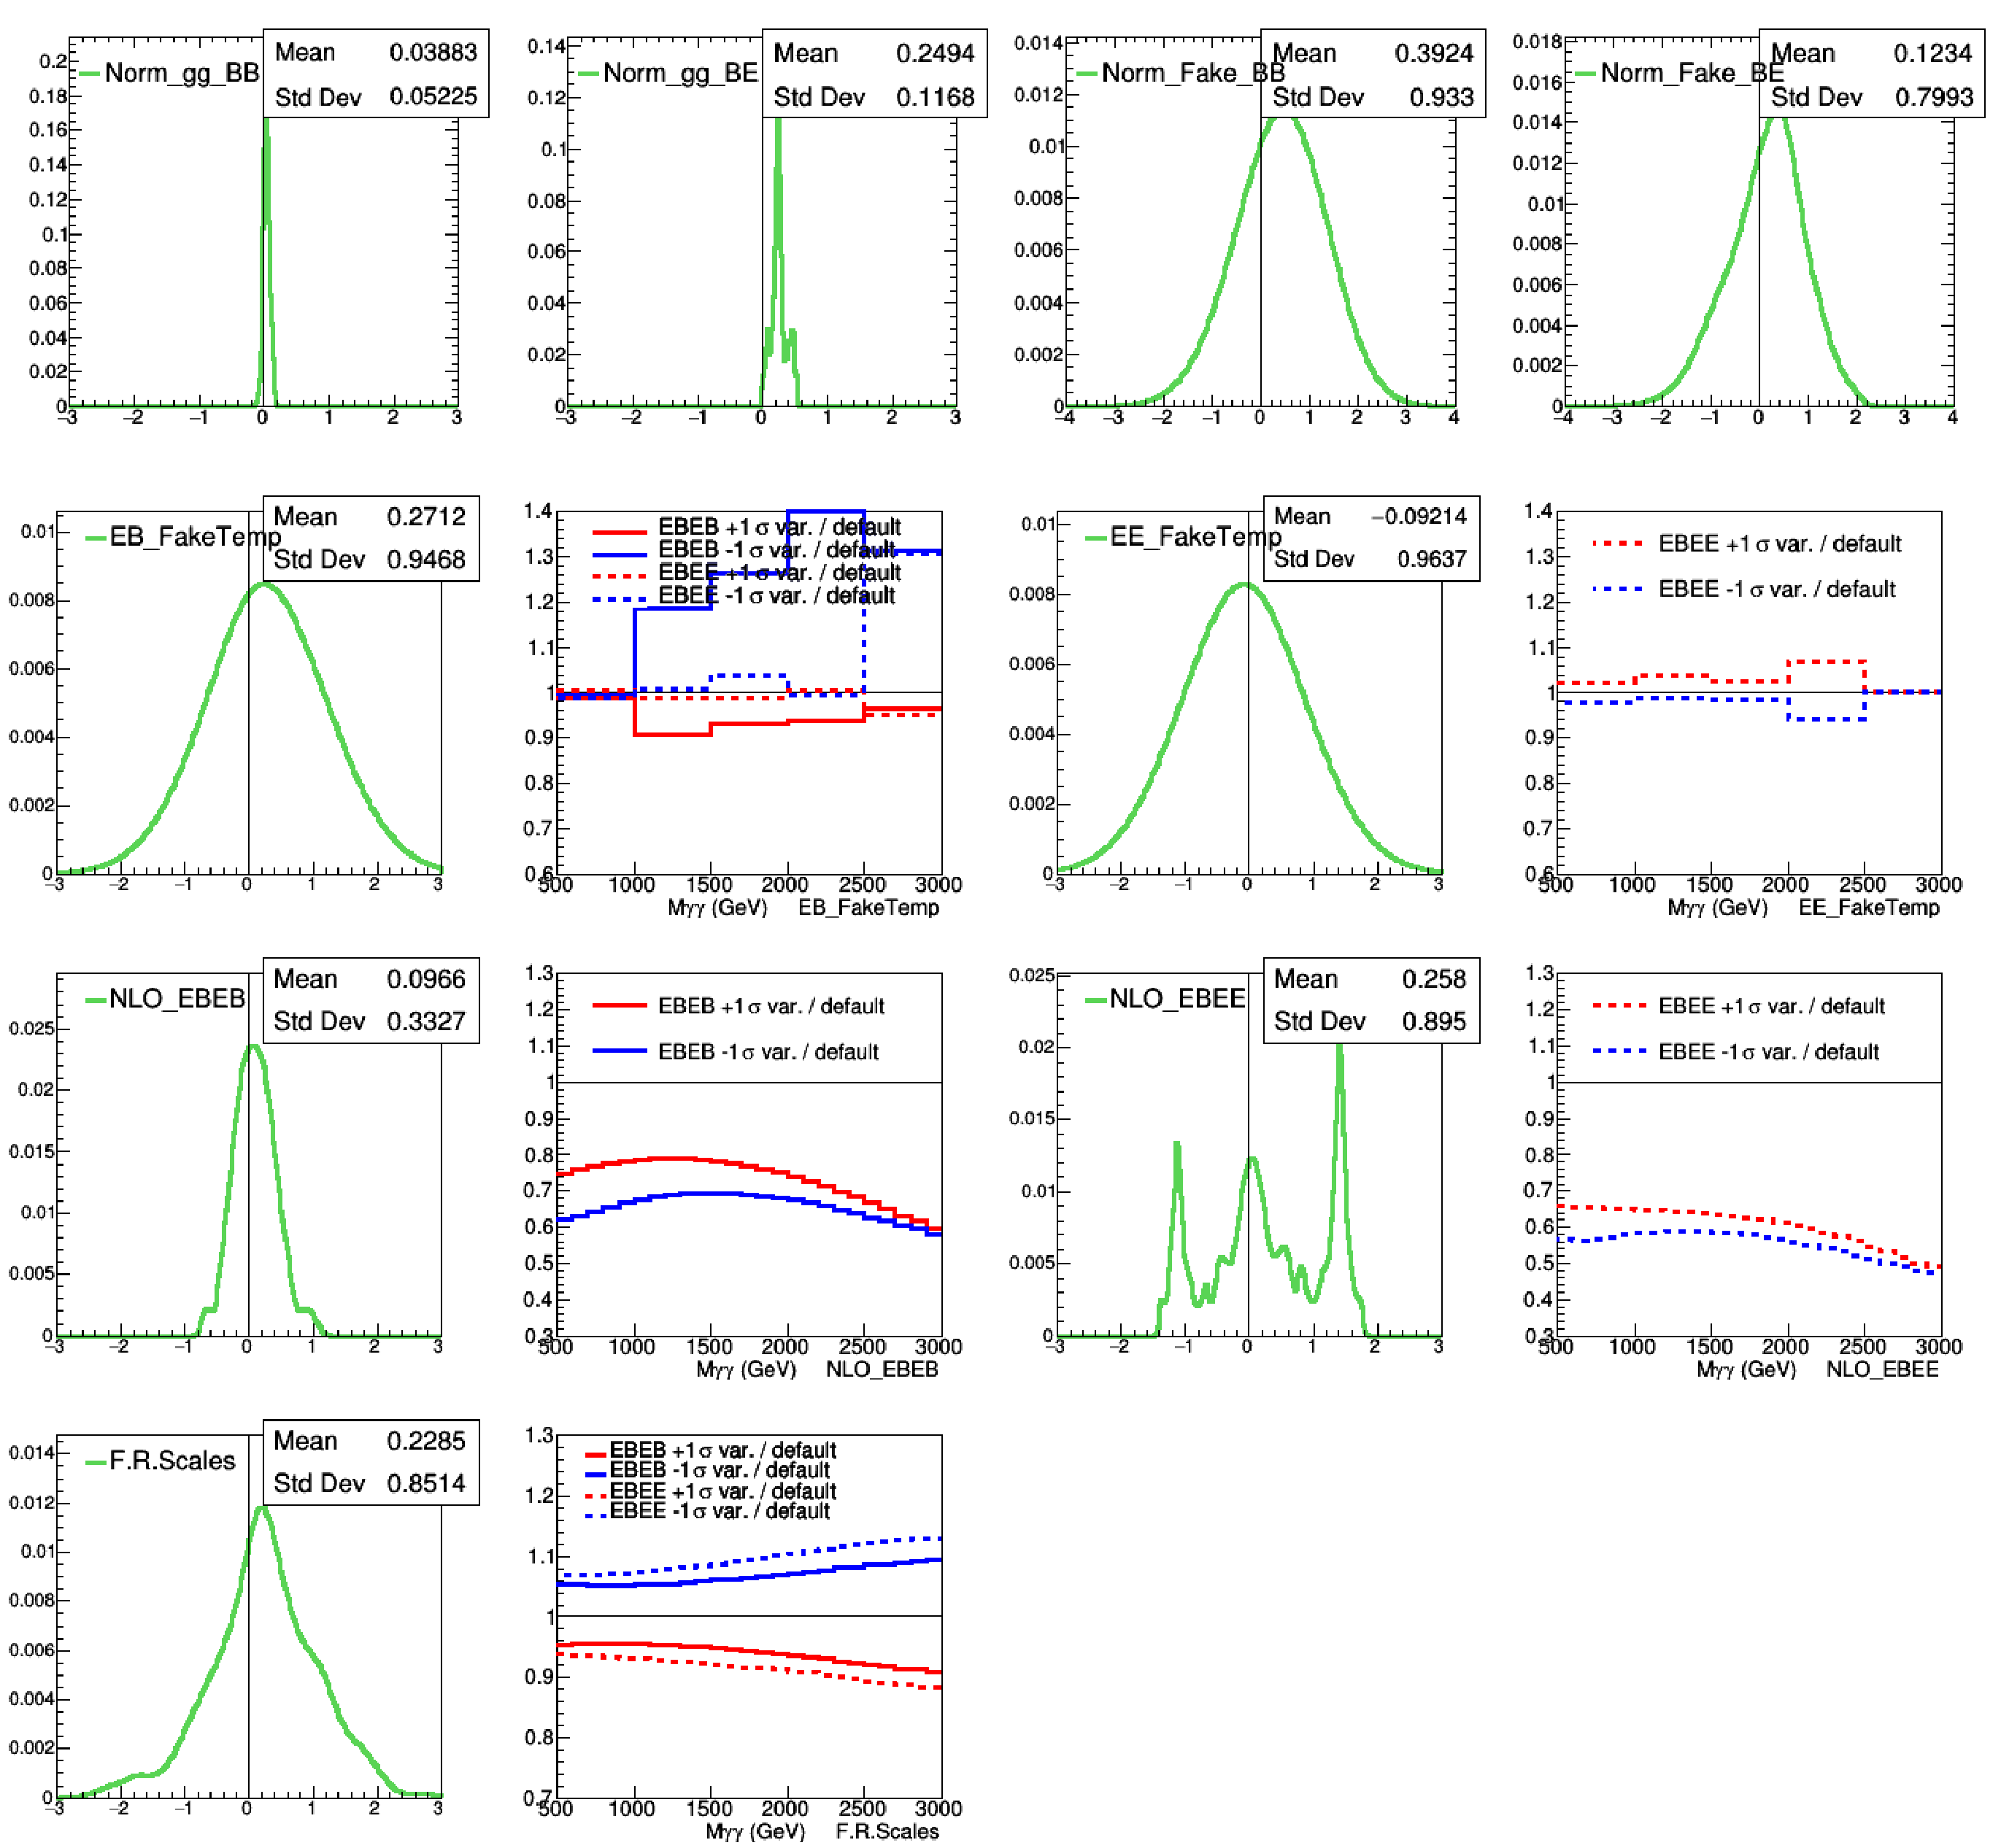
\includegraphics[scale=0.34]{figures/Multi_Rest.pdf}
	\caption{Posterior distributions for all non-PDF nuisance parameters associated with the real and fake backgrounds. Some of their associated $\pm1$ standard deviation variations are shown as a ratio of the variation over the default prediction as a function of \mgg in the EBEB and EBEE categories. These are shown for the normalization of the real and fake background in the EBEB and EBEE categories (first row), the fake templates (second row), the NLO uncertainties (third row), and the factorization and renormalization scale variations (fourth row).}
	\label{fig:Multi_Rest}
\end{figure}

The nuisance parameters are assumed to be fully correlated across the \mgg bins. If a nuisance parameter is uncorrelated between the EBEB and EBEE regions, then separate nuisance parameters are used. For the PDF uncertainties, the eigenvectors are assumed to be fully correlated not only across the EBEB and EBEE regions, but also between the signal and background. The correlation matrix among all nuisance parameters is shown in Fig.~\ref{Fig:corr}. No strong correlation is observed between the PDF eigenvectors. The technique for marginalizing the nuisance parameters was described in the previous section, on the search results. All \mgg spectra used as input to marginalization process are unnormalized, except on the PDF uncertainties for the signal points. \correction{After marginalization, a maximum likelihood estimate is used to determine the posterior background prediction, as well as to provide a posterior prediction on the signal.}


\begin{figure}[!htbp]
	\centering
	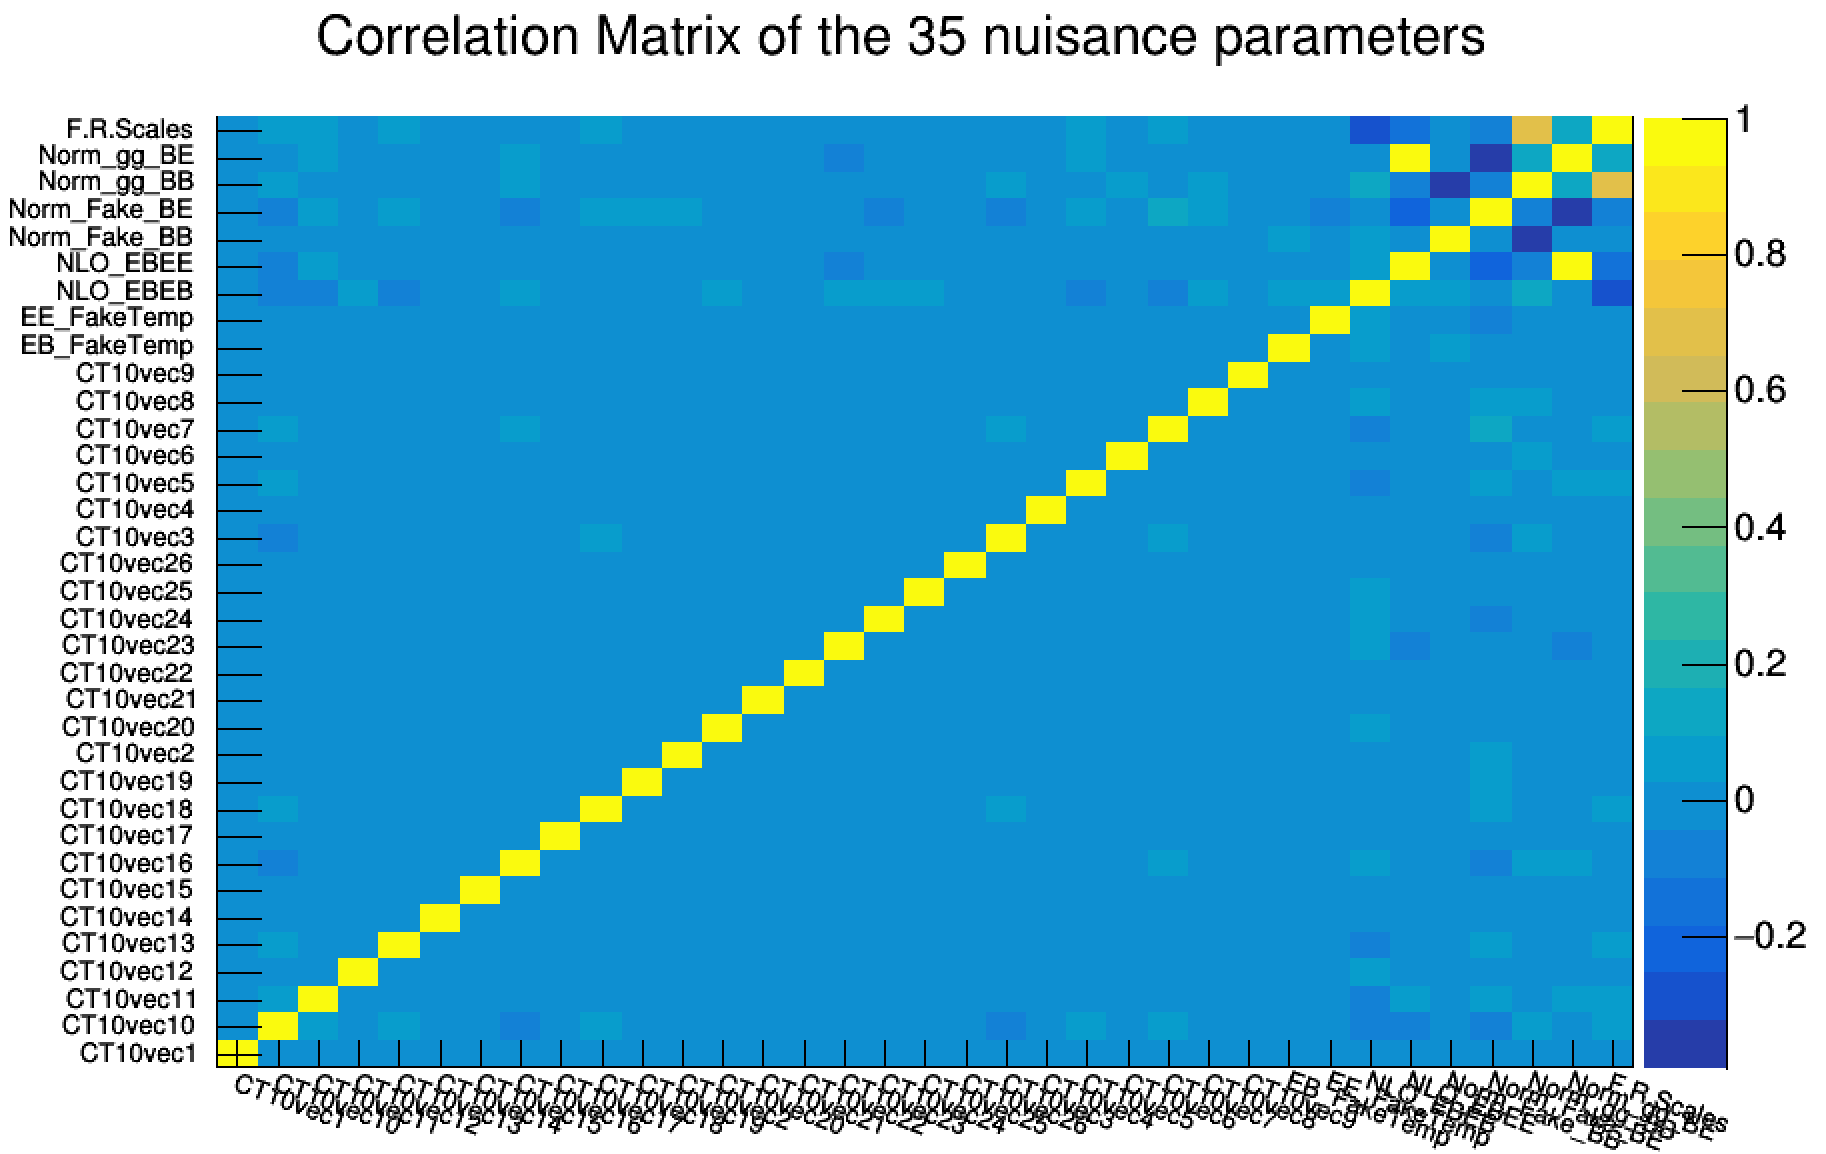
\includegraphics[scale=0.34]{figures/corr35.png}
	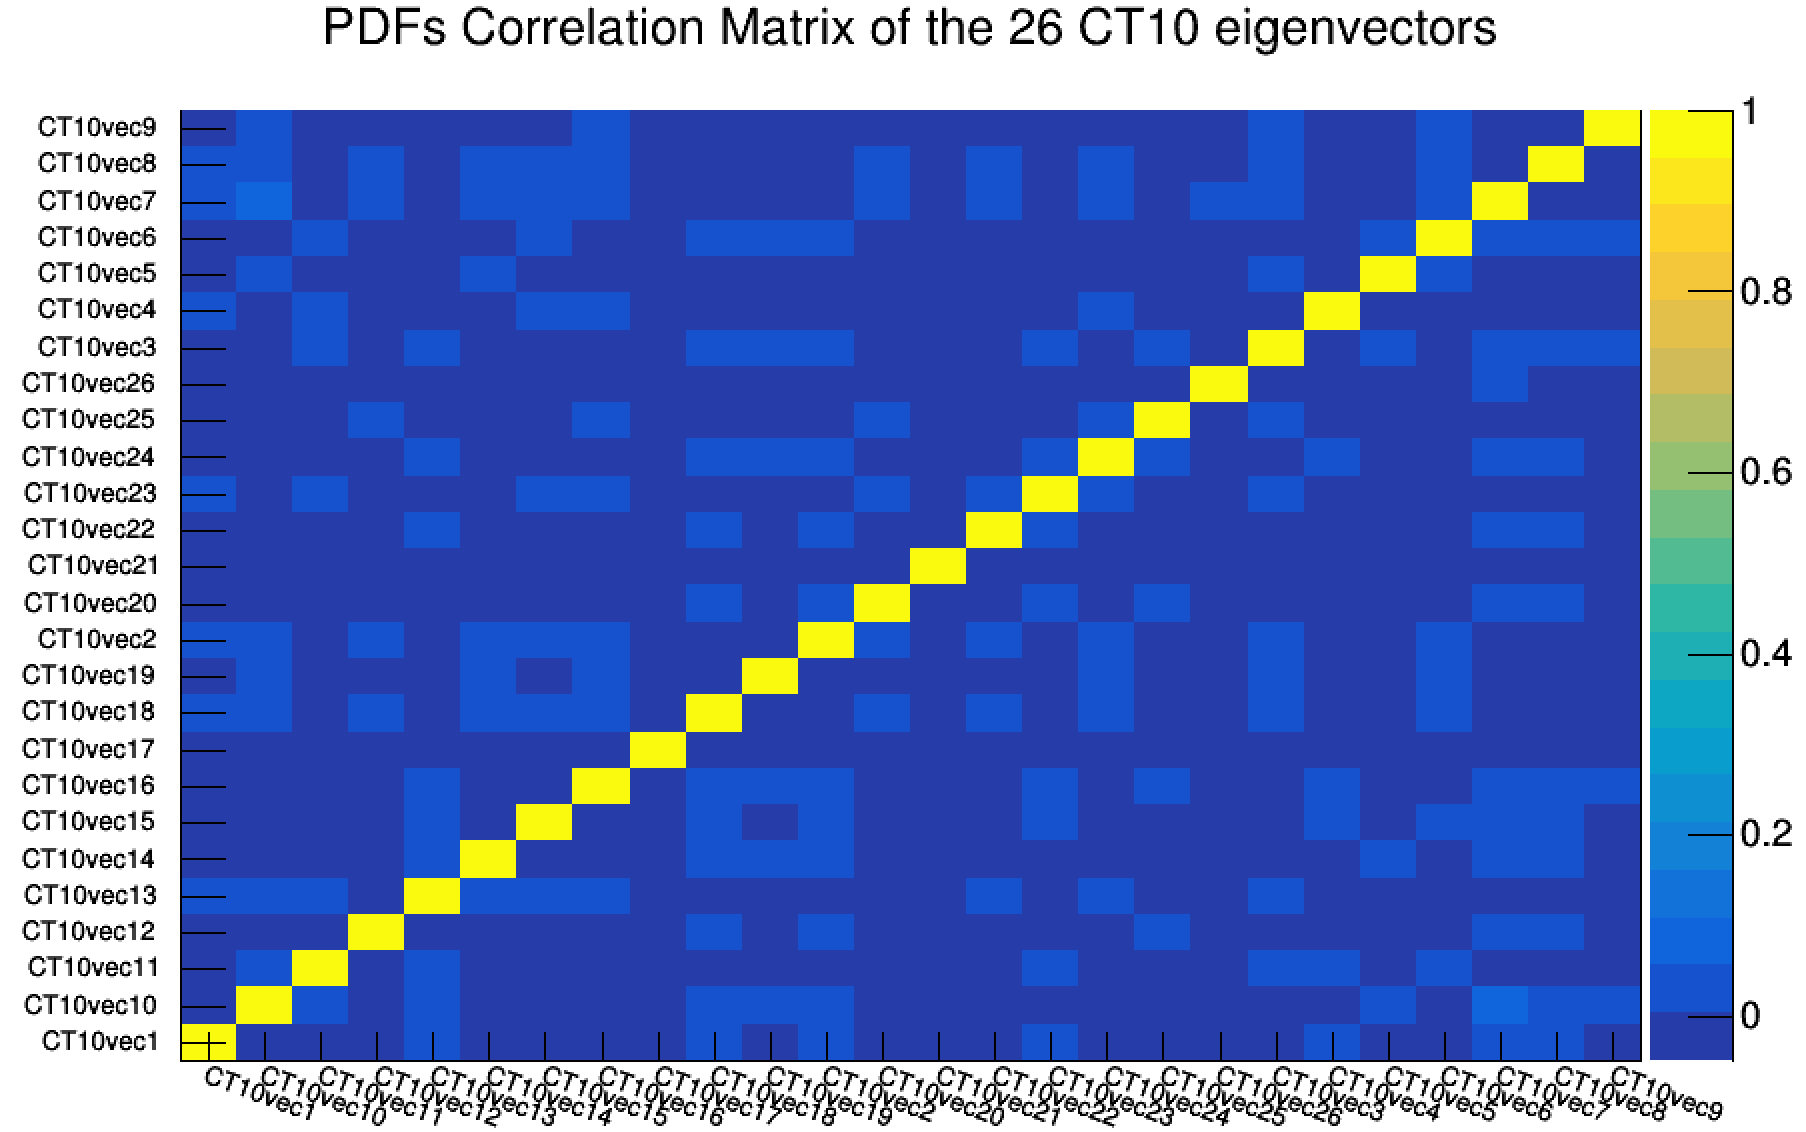
\includegraphics[scale=0.34]{figures/corr26.png}
	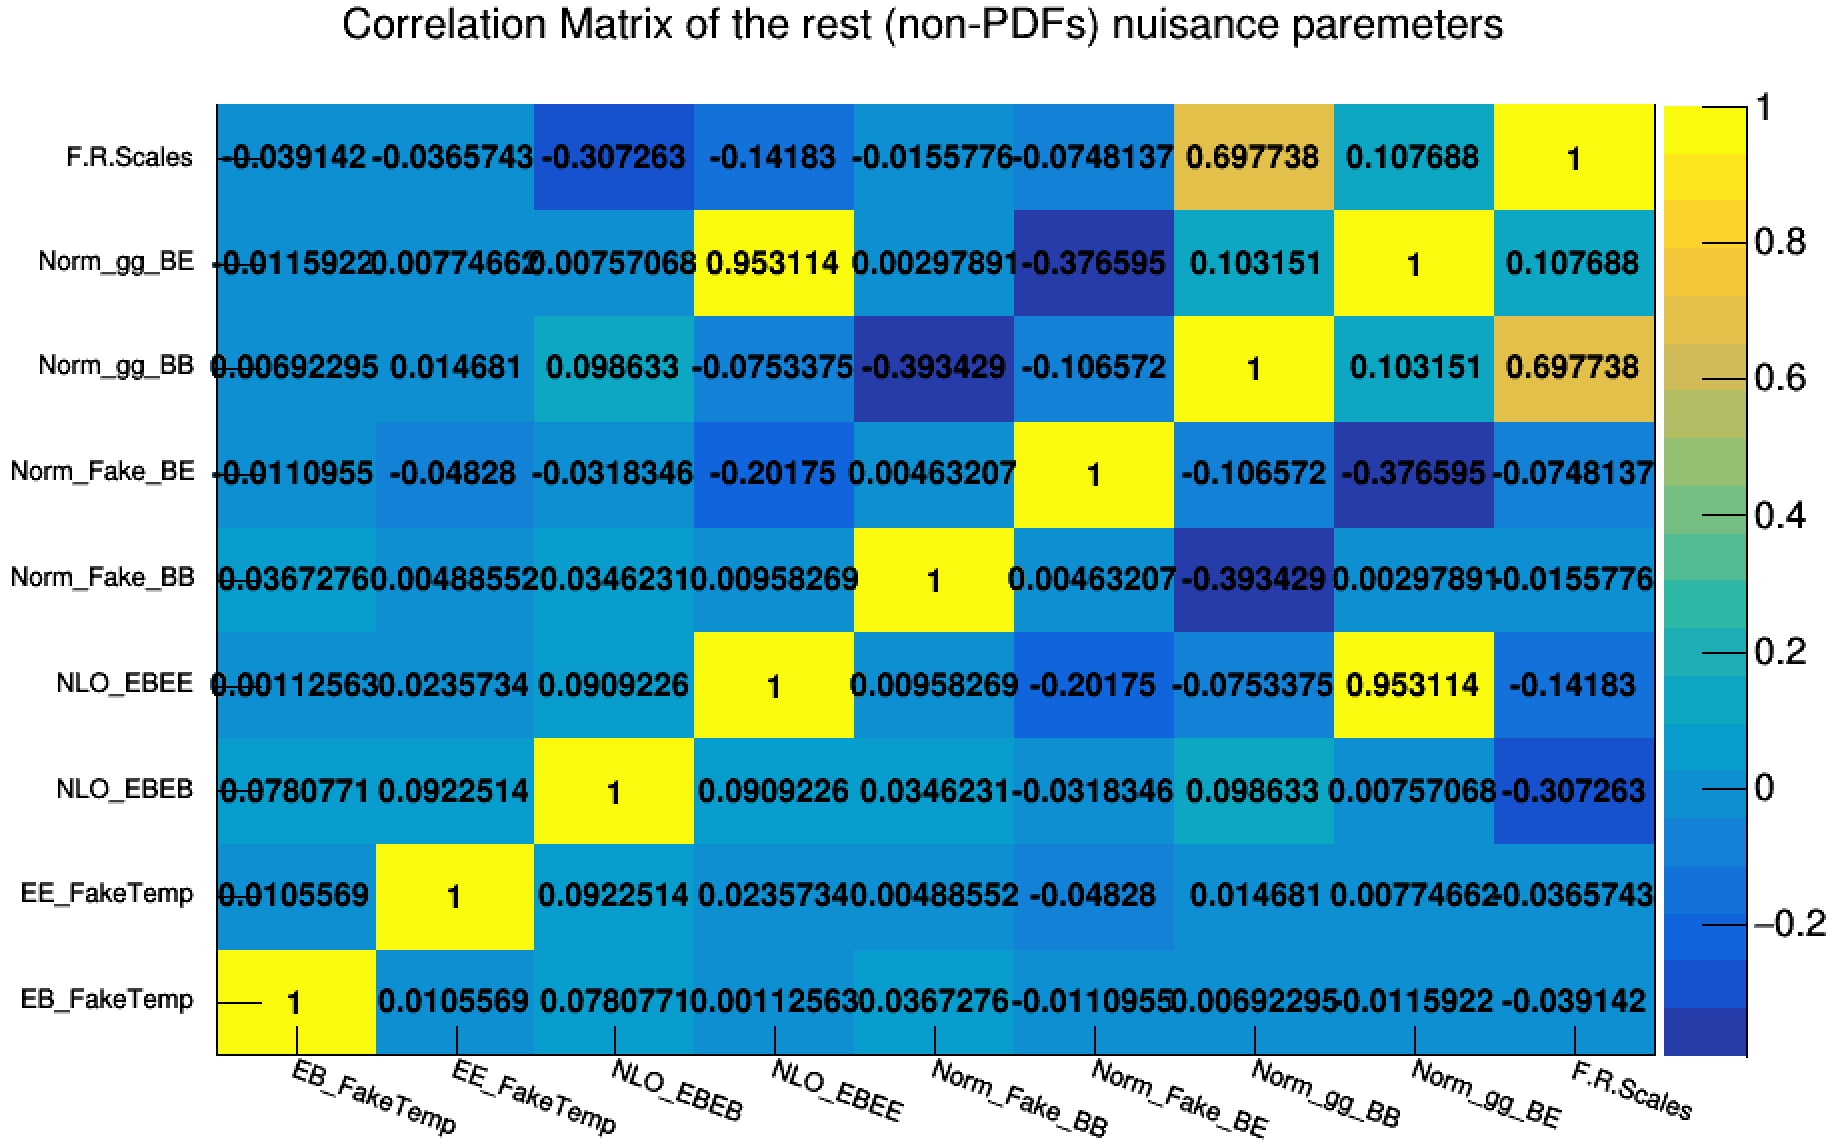
\includegraphics[scale=0.34]{figures/corr9.png}
	\caption{The correlation matrix for all 35 independent nuisance parameters used in marginalization of the real and fake background (top), the 26 PDF nuisance parameters (middle), and the remaining 9 non-PDF nuisance parameters (bottom).}
	\label{Fig:corr}
\end{figure}


\correction{The posterior predictions on the signal are used to derive the Bayesian 95\% confidence level (CL) exclusion limits on the ADD model parameters, in particular, on the parameter \Ms associated with the GRW, HLZ assuming $\nED=2$, and Hewett\texttt{-} model conventions. To determine the 95\% CL upper limits on the signal, we need to integrate the posterior prediction to 95\% of the total integral:}
\begin{equation}
	0.95 = \frac{\int_0^{s^{\textrm{up}}} P(s,b|n)ds}{\int_0^{\infty} P(s,b|n)ds} = \frac{\int_0^{s^{\textrm{up}}} \mathcal{L}(n|s,b)ds}{\int_0^{\infty} \mathcal{L}(n|s,b)ds}
\end{equation}
\correction{where $s^{\textrm{up}}$ is the value of $s$ needed to satisfy this equation. These upper limits are translated into lower limits on the mass scale \Ms by interpolating the value of \Ms that has a signal of 1.0 excluded.}

\correction{One caveat with this approach is that the interference effects between the SM background and ADD signal amplitudes are non-negligible.} Even though the signal is assumed to scale with the normalization, the interference term actually scales as $1/\Ms^4$, while the direct signal term scales as $1/\Ms^8$. Since we are only interested in the signal for a fixed value of \Ms, this approximation has a negligible effect, but, for values of the excluded signal away from 1.0, this cannot be naively extrapolated.

\correction{The 95\% CL exclusion limits on the strength of the signal for the GRW, HLZ assuming $\nED=2$, and Hewett\texttt{-} conventions are shown in Fig.~\ref{fig:ADD_limits}. These limits are expanded to the other ADD model conventions, namely, Hewett\texttt{+} and HLZ assuming $\nED=3$-7, using the \etaG parameterization in order to find equivalent conventions corresponding to a specific value of \Ms, as described in Chapter~\ref{ch:signal}.} The expected and observed lower limits on \Ms for the full ADD model parameter space considered in this analysis are shown in Table~\ref{tab:ADD_limits}. \correction{The expected limits are determined assuming that the data follow the background exactly, while the observed limits are based on the actual data, which can differ. From the observed limits,} the excluded values of \Ms range from 5.6 to 9.7\TeV, depending on the model convention.

\begin{figure}[pt]
	\centering
	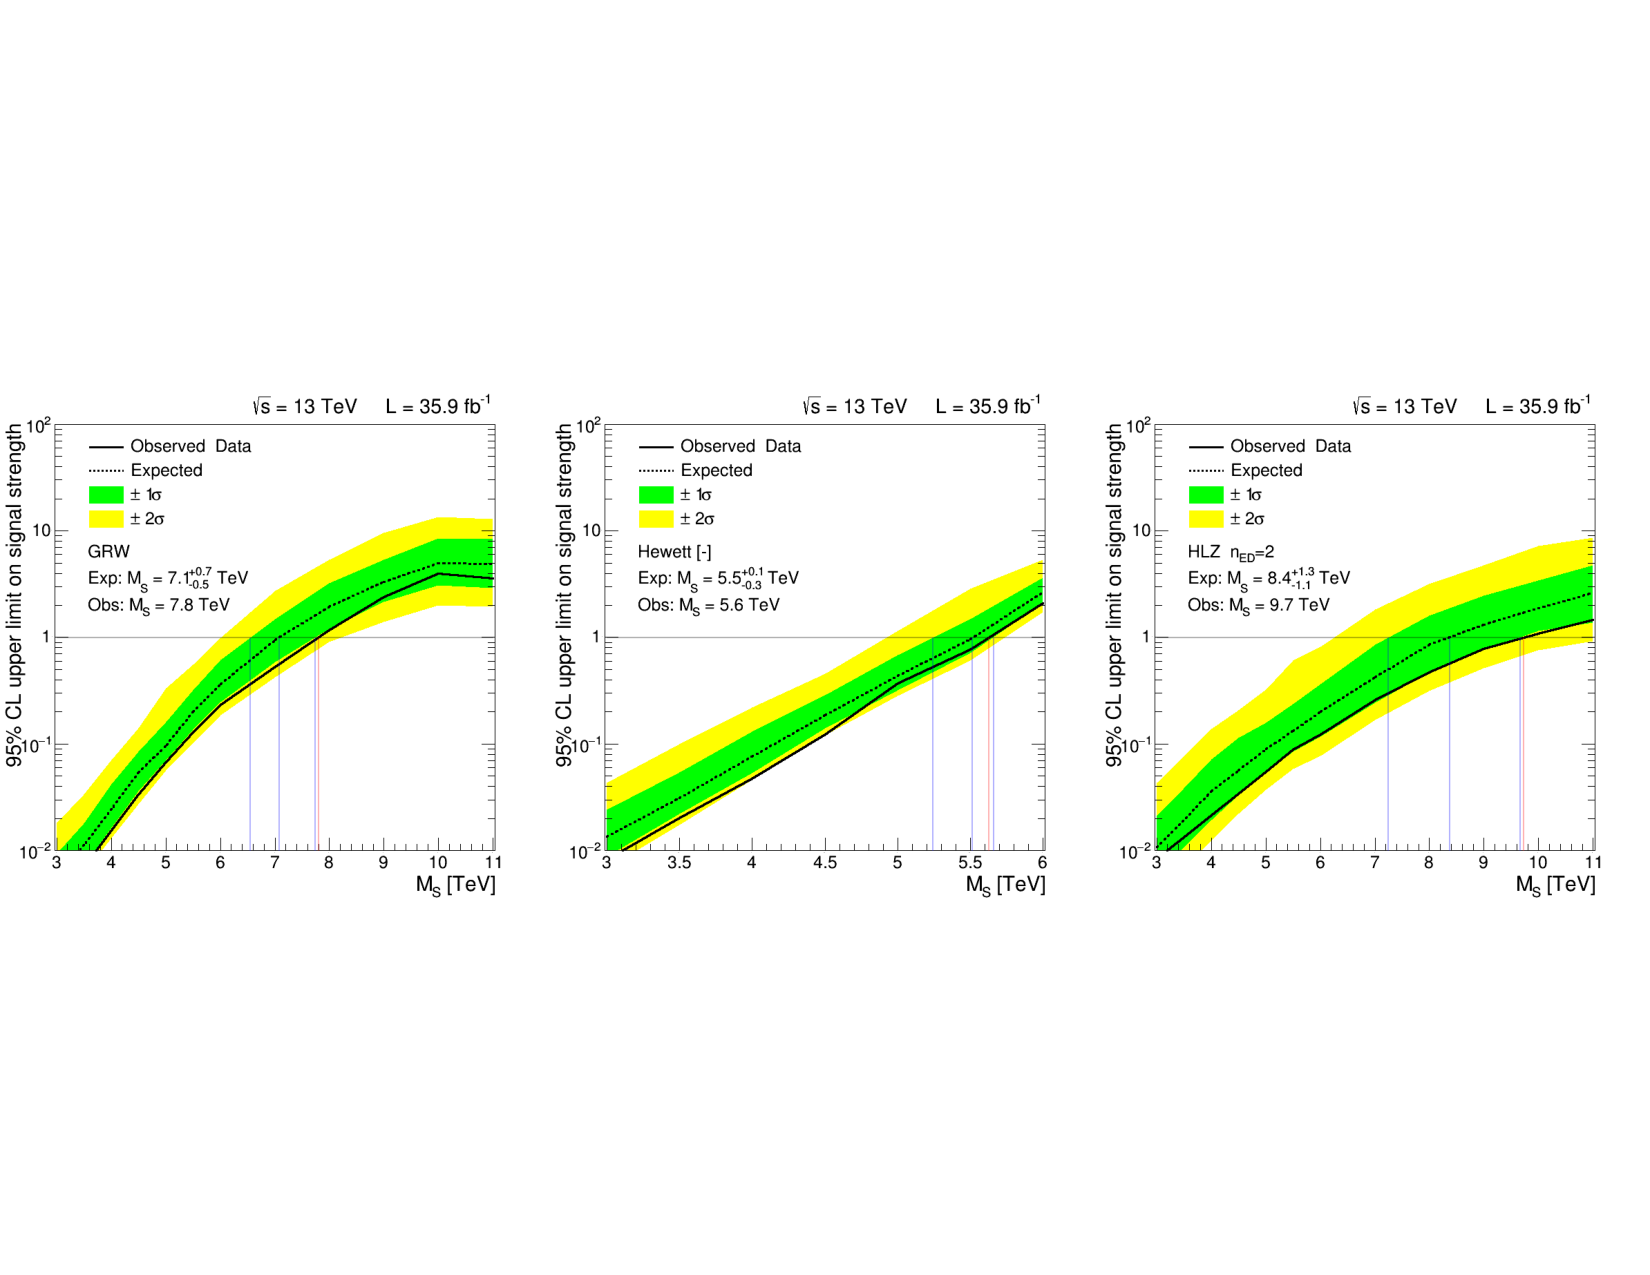
\includegraphics[width=1.0\textwidth]{figures/Multi_Limits.pdf}
	\caption{The 95\% CL exclusion limits on the ADD model signal strength for the GRW (left), Hewett\texttt{-} (middle), and HLZ assuming $\nED=2$ (right) conventions. A 100\GeV binning is used.}
	\label{fig:ADD_limits}
\end{figure}

\begin{table}[pt]
	\centering
	\caption{Exclusion limits on the mass scale \Ms (in units of {\TeVns}) for various conventions used to calculate the ADD large extra-dimensional scenario. The total asymmetric uncertainties are shown on the expected limits.}
	\cmsTable{
	\begin{tabular}{cccccccccc}
		\\	
		\hline \hline
		\vspace*{-3.5mm} &&&&&&&&& \\
		\multirow{2}{*}{Signal} & GRW & \multicolumn{2}{c}{Hewett} & \multicolumn{5}{c}{HLZ} \\
		& & negative & positive & $\nED=2$ & $\nED=3$ & $\nED=4$ & $\nED=5$ & $\nED=6$ & $\nED=7$ \\ [\cmsTabSkip]
		\hline
		\vspace*{-2.5mm} &&&&&&&&& \\
		Expected & $7.1^{+0.7}_{-0.5}$ & $5.5^{+0.1}_{-0.3}$ & $6.3^{+0.6}_{-0.4}$ & $8.4^{+1.3}_{-1.1}$ & $8.4^{+0.8}_{-0.6}$ & $7.1^{+0.7}_{-0.5}$ & $6.4^{+0.6}_{-0.5}$ & $6.0^{+0.6}_{-0.4}$ & $5.6^{+0.6}_{-0.4}$ \\ [\cmsTabSkip]
		Observed & 7.8 & 5.6 & 7.0 & 9.7 & 9.3 & 7.8 & 7.0 & 6.6 & 6.2 \vspace*{1.0mm} \\
		\hline \hline
	\end{tabular}
	}
	\label{tab:ADD_limits}
\end{table}

